\documentclass[a4paper,11pt]{article}
%\usepackage[pdftex]{graphicx}
\usepackage{amsmath}
%\usepackage[latin1]{inputenc}
%\usepackage{hyperref}
%\usepackage[T1]{fontenc}
%\usepackage[utf8]{inputenc}
%%GD Quand je mets usepackage[utf8]{inputenc} je n'arrive plus à compiler la biblio
%J'ai essayé de débuger : je n'y suis pas arrivé
\usepackage{rotating}
\usepackage{setspace}
\usepackage{lscape}
\usepackage[round]{natbib}
\usepackage{multirow}
\usepackage{rotating}
\usepackage{vmargin}
\usepackage{epstopdf}
\usepackage{hyperref}
\usepackage{float}
\usepackage{caption}
\usepackage[tableposition=top]{caption}
\usepackage{amsfonts}
\usepackage{bbold}
% JH : impossible de compiler avec le package bbold, remplacé par amsfonts
\usepackage{upgreek}
\usepackage{comment}
\includecomment{commentGD}
\usepackage[draft]{todonotes}
%\usepackage[disable]{todonotes}
%%GDPour cacher les notes, \usepackage[disable]{todonotes}


%\usepackage[nolists, figuresfirst]{endfloat}
%\usepackage{sidefloat}

\setlength{\abovecaptionskip}{-8pt}

%\usepackage[usenames]{color}
%\definecolor{grey}{rgb}{0.35,0.35,0.35}
%\definecolor{webdarkblue}{rgb}{0,0,0.4}
%\definecolor{orange}{rgb}{0.7,0.2,0.05}


%\usepackage[pdfcreator={PDFLaTeX}, pdfproducer={PDFLaTeX}, pdfstartview=FitH, pdfpagemode=UseOutlines, pagebackref=false, colorlinks={true},
%citecolor={webdarkblue}, linkcolor={webdarkblue},
%urlcolor={webdarkblue}]{hyperref}



%\addtolength{\oddsidemargin}{-0.4in}
%\addtolength{\evensidemargin}{-0.4in}
%\addtolength{\textwidth}{0.8in} \addtolength{\topmargin}{-0.85in}
%\addtolength{\textheight}{1.7in}
\renewcommand{\baselinestretch}{1.2}

\newcommand\cites[1]{\citeauthor{#1}'s\ (\citeyear{#1})}

\newcommand\citeh[1]{\citeauthor{#1}'\ (\citeyear{#1})}

\setmarginsrb{3cm}{2cm}{3cm}{2cm}{0,5cm}{0,5cm}{0,3cm}{0,5cm}



% commands

\newcommand{\bi}{\begin{itemize}}
\newcommand{\ei}{\end{itemize}}
\newcommand{\be}{\begin{enumerate}}
\newcommand{\ee}{\end{enumerate}}
\newcommand{\bd}{\begin{description}}
\newcommand{\ed}{\end{description}}
\newcommand{\beqa}{\begin{eqnarray}}
\newcommand{\eeqa}{\end{eqnarray}}
\newcommand{\beq}{\begin{equation}}
\newcommand{\eeq}{\end{equation}}
\newcommand{\bs}{\bigskip}
\newcommand{\A}{$^a$}
\newcommand{\B}{$^b$}
\newcommand{\C}{$^c$}

\begin{document}



\title{\textsc{Transport costs did decline since 1974:\\Findings from modeling additive costs}\thanks{We are grateful to participants at ETSG 17\textsuperscript{th} meetings in Helsinki, DEGIT XXII in Paris School of Economics, and participants at seminars of the University of California-Irvine, the Universities of Paris-Dauphine Paris-I and Nancy for very useful discussions. Finally, any remaining errors are ours. This paper features an online appendix containing additional results and available on the authors' websites.}}
\author{Guillaume \textsc{Daudin}\thanks{%
Universit\'{e} Paris-Dauphine, PSL Research University, LEDa, 75016 PARIS, FRANCE \newline
Universit\'{e} Paris-Dauphine, PSL Research University, IRD, LEDa, UMR 225, DIAL, 75016 PARIS, FRANCE \newline
Sciences Po, Observatoire Fran\c{c}ais des Conjonctures \'{E}conomiques (OFCE), 75014 PARIS, FRANCE \newline
; email: \url{guillaume.daudin@dauphine.fr}}  \qquad J\'{e}r\^{o}me \textsc{H\'{e}ricourt} \thanks{Universit\'{e} de Lille - LEM-CNRS UMR 9221, France \& CEPII, France; email: \url{jerome.hericourt@univ-lille1.fr}}\qquad Lise \textsc{Patureau}\thanks{Corresponding author. Universit\'{e} Paris-Dauphine, PSL Research University, LEDa, France;  email: \url{lise.patureau@dauphine.fr} } }




%\date{July 2017\\PRELIMINARY AND INCOMPLETE \\ DO NOT QUOTE WITHOUT PERMISSION}

\date{November 2017}
 \maketitle
\bigskip

\begin{abstract}
 In contrast to \cite{hummels2007}, we find that composition effects play a minor role in accounting for the reduction of transport costs relative to the value of US imports. Transport cost ``per se'' did decline. This difference of results can be attributed to the new way of modeling the additive component of transport costs we offer. Exploiting information contained in the US imports flows database over 1974-2013, distinguishing by transport mode (air and vessel), three main results emerge. First, the additive component of transport costs is sizeable, with mean values over the period of 1.8\% and 2.9\% of the export price in air and vessel transport respectively. Second, taking additive costs into account significantly improves the fit of the modeling of transport costs. Third, the modeling of the additive component is key to computing  the decomposition of the trend patterns of transport costs, between what is attributable to trade composition effects and changes in the transport costs for given goods and origins.

\end{abstract}

\thispagestyle{empty} \pagestyle{plain} \setcounter{page}{1}

\bigskip


\noindent \emph{JEL classification}: F14, N70, R40 \\
\noindent \emph{Keywords}: Transport costs estimates, non-linear econometrics, period 1974-2013, additive costs

{\normalsize \vspace{0cm} }

{\normalsize \titlepage }

{\normalsize \newpage }

%\begin{spacing}{1.5}

\section{Introduction \label{sec:Intro}}



\noindent Trade costs are central to international economic analysis. In particular, they are considered a major obstacle to international economic integration and international trade flows. According to \cite{Jacks08}, the trade cost decline explains around 55\% of the pre-World War I trade boom and 33\% of the post-World War II trade boom, while the abrupt rise in trade costs explains the inter-war trade collapse. After 1950, average trade costs fell by 16\%, notably through the reduction of policy trade costs promoted through the GATT (WTO after 1995) multilateral agreements. Based on panel data, \citet{novy13} finds  that U.S. trade costs with major trading partners declined on average by about 40 percent between 1970 and 2000. Yet, several papers (mostly based on empirical estimates of the gravity equation) have shown that trade costs still remain a major obstacle to trade (\citealp{Head_Mayer04} and \citealp{Disdier_Head08}). Using data over 1989-2000, \citet{anderson_wincoop_jel} thus estimate that average international trade costs for industrialized countries represent a 74\% markup over production costs.

Defined as the costs associated with the exchange of goods across national borders, trade costs are usually split between transaction costs (information costs, contract enforcement costs, costs associated with the use of different currencies...), policy costs (tariff  and non-tariff costs), time costs (time to ship goods) and transport costs \emph{per se}. In this vein, \citet{anderson_wincoop_jel} obtain that around 30\% of international trade costs are attributable to transport costs. Equivalently, international transportation costs would represent a 21\% markup over production costs. Further, the sizeable elasticity of trade with respect to freight costs obtained by \cite{Behar_Venables} (around -3) suggests a non-negligible impact of transport costs on trade flows. If much of trade policy barriers have been removed over the second half of the 20th century, these findings point out that the transport costs component of the overall trade costs remain large and deserve attention. This is accordingly the focus of the paper.\smallskip

This focus is shared with part of the international trade literature that studies the patterns of trade costs over time, such as \cite{hummels2007} and \cite{Behar_Venables}. Many argue that transport costs have substantially decreased with technological advance in transportation, infrastructure development and new communication technologies (see \citealp{Lafourcade_Thisse}). \cite{Glaeser04} find that, over the twentieth century, the cost of moving goods have declined by over 90\% in real terms. However, \cite{hummels2007} points out that trade composition effects dominate the characterization of time trends of international transport costs and that, paradoxically, transport costs for given goods and origins have not declined much. We show this result is not robust to a more flexible treatment of additive transport costs. In contrast to \cite{hummels2007}, we thus find that composition effects play a minor role in accounting for the trend patterns of transport costs. \medskip

Following \citet{samuelson1954}, standard models of international trade have usually modeled trade costs as an \emph{ad-valorem} tax equivalent (ie, as a constant percentage of the producer price per unit traded, part of the ``iceberg cost'' hypothesis)\footnote{Rigourously speaking, the ``iceberg cost'' includes both the ad-valorem dimension of trade cost and the fact that these costs are paid in terms of the good that is traded. As this last element is irrelevant in our case, we use the terms ``iceberg'' and ``ad-valorem'' interchangeably, as commonly done in the literature.} However, the structure (additive vs ad-valorem) of transport costs is far from being anecdotal. The literature has long emphasized its role in shaping the pattern of trade flows. As pointed out by \cite{alchian}, the relative price of two varieties of some good will depend on the level of trade costs as long as they display an additive component. In this context, the relative demand for more expensive/higher quality product goods increases with trade costs (``shipping the good apples out''). This is consistent with the findings by \citet{hummels_skiba}, who estimate the elasticity of freight rates with respect to price to be well below unity. Also, their estimates imply that doubling freight costs increases average free alongside (fas) export prices by 80 to 141 percent, consistent with high quality goods being sold in markets with high freight costs. \citet{Lashkaripour-mimeo-2017} challenges this view. Highlighting that more expensive goods are systematically heavier (and hence more costly to transport\footnote{Yet, one can be concerned by the generality of this result. While the positive correlation between weight and price seems reasonable for goods from the second industrial revolution like cars, it is dubious in the case of ITC goods which importance has been rising since the end of the 20\textsuperscript{th} century.}), he finds an average transport cost elasticity much closer to 1 using firm-level data on Colombian imports. This result is also confirmed on more aggregate US, sector-level trade data. The debate is not over yet, as recent empirical studies based on micro-level data conversely provide a strong empirical support to the role of additive costs (i.e., cost per unit exported) in international trade costs. Based on a firm-product-level database of French exporters, \citet{martin2012} finds that firms charge higher unit values for exports to more remote countries, in contradiction with the ad-valorem hypothesis. Recently, \citet{Irrazabal_2015} document on Norwegian firm-level trade data that additive costs represent a sizeable share of international trade costs. Based on US sectoral data, our own estimates also suggest an important part for additive costs in international transport costs.

%\citet{Lashkaripour-mimeo-2017} takes into account the fact
%Yet, one can be concerned by the generality of this result. The positive correlation between weight and price seems reasonable for goods from the second industrial revolution like cars, it is dubious in the case of ITC goods which importance has been rising since 1994 (the end point of Lashkaripour's study). Measurement error in Columbian data??

Beyond the positive aspect, several recent papers also point out the normative implications of additive trade costs. \citet{sorensen2014} extends \citet{melitz}'s seminal model of international trade by including additive trade costs, in addition to the ad-valorem component. A key analytical result is that the welfare gain from a reduction in trade barriers is higher for a decrease in additive costs than a decrease in ad-valorem costs.\footnote{This is due to the alteration of relative prices in a heterogeneous-firms trade framework. Lower additive trade costs reduce the export market prices of the highly performing exporters relative to lowly performing exporters. This, in turn, shifts relative market shares among exporters towards the highly performing ones - a mechanism that can not occur under ad-valorem costs. Total export sales are then reallocated between a smaller number of high-productivity firms. Therefore, the expected profits from exporting prior to entry increase all other things being equal by more in the case of lower per-unit costs, driving up incentives to enter the industry and bringing eventually the welfare enhancing intra-industry reallocations highlighted in \citet{melitz} framework.} Calibrating on Norwegian firm-level data for 2004, \citet{Irrazabal_2015} find that an additive import tariff reduces welfare and trade by more than an identically-sized ad-valorem tariff. While these results suggest that important welfare gains can be achieved by reducing additive trade costs, not much progress has been done in quantifying such gains. One potential reason is the lack of an empirical characterization of the additive component of trade costs.\footnote{The one exception being \citet{Irrazabal_2015}, upon which we come back later.} One objective of the paper is to fill this gap. \bigskip


Do additive costs matter? To answer this question, we provide an empirical decomposition of the structure of transport costs over time, by explicitly distinguishing between ad-valorem and additive parts. To do so, we exploit information contained in the US Imports flows over 1974-2013, from which we get a measure of international transport costs as the difference between the import and the export prices, on a year-product-partner country basis. Obviously, exploiting this database has drawbacks, in particular as it restricts our scope of study to the monetary dimension of international transport costs. Since our measure is based on the gap between export and import prices, it necessarily omits the other dimension of transport costs related to the time value of goods in transit. According to \citet{anderson_wincoop_jel}, the 21\% markup over production costs coming from transport costs includes both directly measured freight costs (10.7\%) and 9\% tax equivalent of ``indirect'' costs related to the time value of goods on their way to their export market (including holding cost for the goods in transit, inventory cost due to buffering the variability of delivery dates, preparation costs associated with shipment size...). Still, the evidence summarized in \citet{anderson_wincoop_jel} points to a persisting importance of direct transport costs, especially compared to other trade barriers. They remain more important than, e.g., policy barriers (8\% tax equivalent), language barrier (7\%) or information cost (6\%). \citet{Hummels_1999} mentions several papers which all point that transport costs pose a barrier similar in size, or larger than tariffs. In the same vein, \citet{limao_venables} highlight the importance of infrastructures for trade costs in general, through their impact on transport costs. Furthermore, our data is based on a single and reliable customs source with a wide time and geographical coverage, and it allows the computation of a direct transport cost measure. This limits the measurement error bias. Therefore, we strongly believe that exploiting this database may deliver useful and reliable insights on the structure of international trade costs.

By investigating the additive dimension of transport costs, our paper is related to the literature that challenges the dominant role of iceberg costs in international trade.\footnote{On top of the previously cited papers about additive costs, our paper also relates to \citet{Alessandria-et-al-AER-2010}, \citet{Hornok-et-al-RES-2015} or \citet{Hornok-et-al-JIE-2015}, which point out the role of per-shipment costs (among which, administrative costs) in generating some ``lumpiness'' in international trade transactions.} Closely related to our paper is the work by \citet{Irrazabal_2015}, which develop a structural framework for inferring additive trade costs from firm-level trade data. Based on Norwegian exports in 2004, they find that the ratio of additive to ad-valorem trade costs is about 14\% of the export price. Our paper complements their findings in two main respects. First, if our study covers a narrower set of trade costs focused on transport costs, our empirical analysis allows us to provide distinct measures of the levels of both the iceberg and the additive trade costs. Second, we exploit exhaustive information about the imports flows of the US over a large time span from 1974 to 2013. In this respect, our results deliver a broader view of the magnitude of additive costs in international trade over time. Despite these differences, our results share with \citet{Irrazabal_2015} the important role of the additive component of international trade costs.\smallskip

Our three main findings can be summarized as follows. First, we show that additive costs are quantitatively sizeable. On average over 1974-2013, the additive cost is estimated to 1.8\% and 2.9\% of the export price in air and vessel transport respectively. This is slightly lower than our estimates for the ad-valorem component (3.5\% and 3.2\% for air/vessel respectively on average over the period). Put it differently, additive costs represent between 40 \% and 50\% of the overall transport costs, depending on the year and the transport model. To the best of our knowledge, our paper is the first to provide such an extensive quantitative measure of both ad-valorem and additive costs in total transport costs.\footnote{Given their database and their empirical approach, \citet{Irrazabal_2015} can only identify the ratio of the additive to the ad-valorem cost ($\frac{t_{ik}}{\tau_{ik}}$ in our terminology), that they interpret by expressing it in terms of the median export price by country-product ($\bar{\widetilde{p}}_{ik}$). By contrast, our estimation strategy enables us to uncover both values of the ad-valorem and the additive costs $\tau_{ik}$ and $t_{ik}$ separately, in terms of the country-product export price $\widetilde{p}_{ik}$.}. This represents a valuable insight for calibrating related international trade or business cycle models.

Second, we provide an empirical assessment of what standard international trade models lose by skipping additive transport costs. Quantitatively, the omission of the additive term leads to overestimate the ad-valorem component by roughly a factor 2. On average over the whole period, biased estimates for ad-valorem are 5\% for air and 6\% for vessel, while unbiased estimates are respectively 2.5\% and 3.2\%. Further, we obtain a systematically better goodness of fit when the additive component is included in the regression, even when taking into account the additional degrees of freedom.

Third, additive costs matter in accounting for the time trend of transport costs, as we show by exploiting the time dimension of our database to document the patterns of transport costs over time. Between 1974 and 2013, we thus find that transport costs have decreased by roughly 50\% in air shipping and 60\% in vessel shipping, and of same order of magnitude for both additive and iceberg components. Importantly, we find that most of this decline can be attributed to a reduction in the ``ceteris paribus'' transport costs, rather than to trade composition effects, in contrast to the conclusion obtained by \cite{hummels2007} on the same database (until 2004). Importantly, we show that the difference of results can be attributed to the modeling of the additive component: Allowing the additive costs to vary over the triple time/product/country partner case (rather than being constant as in \cite{hummels2007}), turns out to be key in the decomposition of underlying sources of the decrease of overall transport costs observed over the period. In all three aspects, our results thus point the importance of the additive component in accounting for international transport costs.\smallskip

The paper is built as follows. Section \ref{sec:data_method} presents our data and our methodology. In Section \ref{sec:results_decomposition}, we provide results about the size and the role of the additive component of transport costs. After reporting the mean values over the period (by transport mode), we show how introducing additive transport costs improves the modeling of transport costs. Section \ref{sec:results_trends} characterizes the trends of transport costs (by transport mode) over the period 1974-2013. Section \ref{sec:robustness} provides some additional robustness checks of our results. Section \ref{sec:conclu} concludes.



\section{Data Sources and Empirical Methodology \label{sec:data_method}}

\subsection{A measure of transportation costs}

Our analysis of transportation costs consists in exploiting the difference between commodity-level export and import prices, as in \cite{hummels2007} (among others). The database we use to construct our measure of transport costs comes from US annual Imports of Merchandise provided by the Census bureau,\footnote{More information available at: \url{http://www.census.gov/foreign-trade/reference/products/catalog/fl_imp.txt}} spanning from 1974 to 2013. We first use customs values, quantities and freight costs to recover free-alongside (fas) and cost-insurance-fret (cif) prices, by goods, country of origin and transportation mode.\footnote{The related literature commonly refers to the fob price rather than the fas price. While both are closely related, we refer to the fas price as the price considered by the US Foreign Trade Statistics.} More precisely, the (unit) fas price is computed as the total ``customs value'' in the US trade statistics divided by the shipping weight; in other words, it is the price for one kg of the good net of transportation costs. The cif price is then computed as the sum of the customs value and freight charges, once again divided by the shipping weight. Our dependant variable is finally computed as the ratio of the cif price divided by the fas price. Higher than 1, the variable provides a measure of transport costs as a proportion of the good's price, an \emph{ad-valorem} equivalent. This is a quite standard and widespread strategy, as emphasized by \citet{anderson_wincoop_jel}.

Obviously, this dataset is not immune of limitations. First, it restricts our analysis to the study of international transport costs, as our measure of the cif-fas price gap only covers freight, insurance and handling costs. It is thus silent about the others dimensions of international trade costs, unlike \citet{Irrazabal_2015}. Further, in terms of transport costs \textit{per se}, our measure based on the cif-fas price gap captures the quantitative costs due to insurance, handling and freight, but it omits the other dimension of transport costs related to the time value of goods in transit. In this respect, this dataset embraces only a partial view of international transport barriers. However, it is also clear that direct transport costs do represent a sizeable share of trade costs as pointed out in Section \ref{sec:Intro}. Last, as mentioned by \cite{Lafourcade_Thisse}, our transport costs measures is based on actual trade flows, i.e. ignoring those flows that did not happen because of presumably prohibitive transport costs. In light of this, the estimated values that we obtain can be viewed as the lower bounds of the ``true'' transport costs. %JH: OK, parfaitement clair pour moi !

Yet, this dataset also has (at least) three advantages. First, it delivers a strong statistical reliability arising from a single, homogenous and trustworthy customs source. Based on customs declarations, the US Imports database inventories all imports (both values and quantities), by country of origin, to the United states at the HS 10-digit level, with a concordance code to the SITC 5-digit coding system. This will be crucial to compute transport costs, as we detail below. In addition, the database reports information regarding freight, insurance and handling expenditures by transportation mode, ocean (or ``vessel'') and air. We will make use of this to enlighten potential differences in the dynamics of transport costs across transportation mode. Second, using this dataset allows us to have both the import price and the export price for the same good (for a given origin country). This is highly valuable, as it gives us a direct measure of international transport costs (at the country/sector level), from which we can estimate separately the \textit{levels} of both the iceberg costs and of the additive costs. Third, this dataset is available over a long time span, which we exploit by providing an analysis of the trend patterns of international transport costs over the period 1974-2013. \smallskip

We estimate international transport costs at the 3-digit classification level, even if data series on the cif and fas prices are available at the 5-digit classification level. As detailed below, the use of a nonlinear estimator triggers computational limitations that limit the level of possible detail, especially when covering a long period of time. Yet, we ensure the robustness of these results by conducting the estimations at the 4-digit level for some selected years.\footnote{The selected years for the 4-digit level estimations are: 1974, 1977, 1981, 1985, 1989, 1993, 1997, 2001, 2005, 2009, 2013. Comparing different levels of aggregation is useful to check differences and the presence of biases precisely due to aggregation. However, we obtain no substantial difference between the estimation results conducted at the 3 and 4-digit levels. Estimation results at the 4-digit classification level are reported in Appendix \ref{app:4digit}.} Depending on the considered year, this leaves us with around 200 sectors, from approximately 200 countries of origin.



\subsection{Empirical specification}

\paragraph{The estimated equation} Our purpose is to provide time-varying estimates of the size of ad-valorem and additive costs among total transport costs. To do so, we start from the equation that expresses the price $p$ of a good paid by the importer (import, or cif price) as a function of the producer price $\widetilde{p}$ (export, or fas price), given both per-kg ($t$) and ad-valorem ($\tau$) transport costs, according to:

\begin{equation}
p = \tau \widetilde{p}+ t \label{eq:base}
\end{equation}

\noindent As usual in the literature, the iceberg trade costs are denoted $\tau$ (with  $\tau \geq 1$, $\tau=1$ meaning no ad-valorem trade costs), while additive trade costs are labeled $t$ (with $t \geq 0$, $t=0$ implying no additive costs).  Let us denote $i$ the origin country, and $k$, the product (at the 5-digit level). Transforming the above equation (\ref{eq:base}) as ratio in order to get the percentage change in prices induced by transportation, we thus get the following baseline specification at the root of our estimation (skipping the year and transport-mode dimensions in the notations for reading convenience):
%\footnote{\textbf{Why do we consider the ratio not the difference, with cif price on the LHS and p fas RHS? To be answered?}}

\begin{equation}
\frac{p_{ik}}{\widetilde{p}_{ik}} -1 = \tau_{ik} -1 +\frac{t_{ik}}{ \widetilde{p}_{ik}} \label{eq:base_estimee}
\end{equation}

\paragraph{Estimation Strategy} We follow \citet{Irrazabal_2015} by considering that \textit{i)} both ad-valorem and additive costs are separable between the origin country ($i$) and the product ($k$) dimensions, and \textit{ii)} this separability is in a multiplicative way for the former and an additive way for the latter. In other words, $\tau_{ik}$ and $t_{ik}$ from Equation (\ref{eq:base_estimee}) are written as:\footnote{Notice that, given the magnitude or order of transport costs, assuming an additive or a multiplicative form does not make a substantial difference since, for small values (as we obtain), we have $\tau_i\times \tau_k -1 \simeq (\tau_i-1) + (\tau_k -1)$ and $t_i+t_k\simeq (1+t_i)\times(1+t_k)-1$.}

\begin{eqnarray}
\tau_{ik} &=& \tau_{i} \times \tau_{k} \label{eq:ad-valorem}\\
t_{ik} &=& t_{i} + t_{k} \label{eq:add}
\end{eqnarray}

\noindent As a result, our underlying structural equation is specified as:

\begin{equation*}
\frac{p_{ik}}{\widetilde{p}_{ik}}-1 =\tau_{i} \times \tau_{k} -1 +\frac{t_{i} + t_{k}}{ \widetilde{p}_{ik}} \label{eq:theory_equation}
\end{equation*}

The ratio $\frac{p_{ik}}{\widetilde{p}_{ik}}$ has a lower bound of one, since by construction, the cif price $p$ cannot be lower than the fas price ($p_{ik}>\widetilde{p}_{ik}$). Taking into account this constraint in the estimate suggests that the error term should be always positive and multiplicative, as in:

\begin{equation*}
\frac{p_{ik}}{\widetilde{p}_{ik}}-1 =\left(\tau_{i} \times \tau_{k} -1+\frac{t_{i} + t_{k}}{\widetilde{p}_{ik}} \right)\times \exp(\epsilon_{ik})
\end{equation*}
\noindent where $\epsilon_{ik}$ follows an normal law centered on 0. Considered in logs, the above equation becomes:

\begin{equation}
\ln\left(\frac{p_{ik}}{\widetilde{p}_{ik}}-1 \right)= \ln \left(\tau_{i} \times \tau_{k}+\frac{t_{i} + t_{k}}{\widetilde{p}_{ik}}-1 \right) + \epsilon_{ik} \label{eq:equation0}
\end{equation}

The non-linearity of Equation (\ref{eq:equation0}) implies that it cannot be estimated using standard linear estimators. All estimates are thus performed using non-linear least squares.\footnote{The basis of the method is to approximate the model by a linear one and to refine the parameters by successive iterations. The intuitive criterion for convergence is that the sum of squares of residuals does not increase from one iteration to the next. See \cite{Woolridge-Book-2001} for more details.} Yet, the use of a nonlinear estimator triggers computational limitations that limit the level of possible detail, especially when covering a long period of time. Confronted to this arbitrage, we estimate international transport costs at the 3-digit level as our benchmark classification, even though data series are available at the 5-digit classification level ($k$). In other words, this amounts making the additional assumption, that all products $k$ in a 3-digit sector $s$ share the
same structure of costs.\footnote{We provide a decomposition variance exercise on the observed cif-fas price. As reported in Appendix \ref{app:decomp_variance}, the share of the observed variance that is accounted for by the between-sector ($s$) variance is roughly similar to the between-product ($k$) variance.} This drives us to estimate a modified version of Equation (\ref{eq:equation0}), specified as:
\begin{equation}
\ln\left(\frac{p_{ik}}{\widetilde{p}_{ik}}-1 \right)= \ln \left(\tau_{i} \times \tau_{s(k)}+\frac{t_{i} + t_{s(k)}}{\widetilde{p}_{ik}}-1 \right) + \epsilon_{ik} \label{eq:model_IetA}
\end{equation}
where $\tau_{i}$, $\tau_{s(k)}$, $t_{i}$ and $t_{s(k)}$ are the parameters to be estimated, i.e., fixed effects specific to each origin country $i$ and sector $s$ (at the 3-digit classification level), and $\epsilon_{ik}$ the residual centered on 0. To eliminate the potential influence of outliers, we excluded 5 percent of the upper and lower tails of the distribution in the regression variables. These cut-offs are aimed at eliminating reporting or coding errors. We estimate this equation for each year over the period 1974-2013, for each of the transportation mode reported (air or vessel), on a sectoral-origin country basis ($i,s$). Depending on the year considered, this leaves us with around 800 fixed effects to estimate by transport mode (at the 3-digit level).   \smallskip

One key objective of the paper is to characterize the importance of additive costs relatively to ad-valorem costs. A natural way to answer this question is to perform estimations of Equation (\ref{eq:model_IetA}) constraining additive costs to be equal to zero, and compare the fitting properties and the explanatory power of the models. For each year and transport mode, we thus estimate two models: \textit{(a)} when additive costs are excluded, in which case transport costs are modeled as iceberg costs only (Equation (\ref{eq:model_nlI})), and \textit{(b)} when transport costs are decomposed in the two additive and ad-valorem dimensions (Equation (\ref{eq:model_IetA})). Under Model (\textit{(a)}), the estimated equation simplifies as:\footnote{One may also object that a comprehensive study of the structure of transport costs should also include the third model with only additive costs. This has driven us to estimate this model as well, in which case the estimated equation is written according to: $\ln\left(\frac{p_{ik}}{\widetilde{p}_{ik}}-1 \right)= \ln \left(\frac{t_{i} + t_{s(k)}}{\widetilde{p}_{ik}}\right) + \epsilon^{add}_{ik}$. The main result that emerges is that the model with additive costs only is dominated (in terms of quality of fit properties) by the model with multiplicative costs only (Equation (\ref{eq:model_nlI})), which is itself dominated by the complete model (Equation (\ref{eq:model_IetA})), anticipating on further results. These results are reported in the Online Appendix, available on the authors' webpages.}

\begin{equation}
\ln\left(\frac{p_{ik}}{\widetilde{p}_{ik}}-1 \right)= \ln \left(\tau_{i}\times\tau_{s(k)}-1 \right) + \epsilon^{ice}_{ik} \label{eq:model_nlI}
\end{equation}

One may be concerned that the specification of Equations (\ref{eq:model_IetA}) or (\ref{eq:model_nlI}) might be subject to endogeneity bias, as the price set be the exporter may vary depending on the transport cost burden. Studies on the pricing-to-market behavior of firms (see \citealp{Krugman-87}) show that we cannot exclude that the export price set by the firm ($\widetilde{p}_{ik}$) is partly endogenous to the size of transport costs (for instance, the exporting firm absorbing (part of) the transport costs by reducing the fas price). However, we consider as a reasonable assumption that the exporting firm cannot influence the international transport cost sector, as that would imply some a direct influence between the firm's prices and the size of transport costs, except in the choice between air and vessel transport (that is beyond our scope of analysis). Otherwise stated, conditional to an export price and a transport mode, the gap between the export price declared to the custom data and the import price recorded by the US administration is beyond the firm's control. In this respect, we are confident that our estimation strategy is immune from endogeneity problems. \smallskip


After estimating Equation (\ref{eq:model_IetA}), we can re-built a measure of each component, $\widehat{\tau}^{adv}_{is} = \widehat{\tau_{i}} \times \widehat{\tau}_{s(k)}$ for the ad-valorem cost and $\widehat{t}_{is} = \widehat{t}_{i} + \widehat{t}_{s(k)}$ for the additive cost, that are country-sector specific, by year and transport mode. When assuming iceberg costs only (Equation (\ref{eq:model_nlI})), we proceed similarly to get $\widehat{\tau}^{ice}_{is} = \widehat{\tau}_{i} \times \widehat{\tau}_{s}$.\footnote{In this case, notice that the equation could be estimated relying on a linear form. To preserve comparability of the results, we keep the same non-linear estimation method in both cases though.} Similarly as \citet{Irrazabal_2015}, we take the average over the sector-country dimension, using the values of each trade flow ($is$-specific) over total yearly trade as a weighting scheme. We thus recover a ``synthetic estimate'' of each type of transport cost: \textit{a)} $\widehat{\tau}^{ice}$, \textit{b)} $\widehat{\tau}^{adv}$ and $\widehat{t}$, for each year and transportation mode. These results are reported in Section \ref{sec:results_decomposition}.

%\textbf{mettre les 3 modeles dans la online appendix.}

\section{Decomposing Transport Costs: The importance of the additive component \label{sec:results_decomposition}}

Do additive costs matter? This section provides two elements of answer to this question. First, we quantify the magnitude of transport costs over time (by transport mode), distinguishing whether the additive component $t_{ik}$ is excluded or included in the estimated equation (Equation (\ref{eq:model_IetA}) or (\ref{eq:model_nlI})). This allows us to estimate whether additive costs represent a sizeable component of transport costs. Second, we assess the importance of the additive component of in overall transport costs through goodness-of-fit measures.


\subsection{Decomposing transport costs over 1974-2013}

Our first contribution to the literature is to provide estimates for the size of both the ad-valorem and the additive components of transport costs. Table \ref{tab:summary_results} reports a summary of our results. It displays the mean and median values of each type of transport costs (either ad-valorem estimated alone or estimated along with additive costs), as well as the associated standard deviation, averaged over the period 1974-2013, for estimation driven both at the 3- and 4-digit sectorial level for different specifications and data. The first panel reports the results for a specification based on ad-valorem costs estimated alone (Equation (\ref{eq:model_nlI})), while the second panel presents estimates for a specification involving both ad-valorem and multiplicative components (Equation (\ref{eq:model_IetA})). Finally, the third panel reports the same set of descriptive statistics, but for the actual cif/fas ratio in our data.\footnote{In Appendix \ref{app:more_results}, we report similar results for a sample of years, for both transport mode, at the 3 and 4-digit classification level. Results for all years (available at the 3-digit level) are reported in the Online Appendix, available on the authors' webpages.}$^{,}$\footnote{We present the estimation results for Air at the 3-digit level removing the year 1989, as the results reveal the presence of strong outliers that bias the estimates of transport costs upwards this particular year. Overall results (over the whole period) are not substantially affected if this year is included though. This can be uncovered from the results detailed year by year in the Online Appendix, available on the authors' webpages.}

\begin{table}[htbp]
  \centering
  \footnotesize{
  \caption{Transport costs estimates: Summary \label{tab:summary_results}}
  \begin{center}
    \begin{tabular}{l|cc|cc}
      \hline \hline
    \multicolumn{5}{c}{Mean value over 1974-2013}   \\
    \# digit & \multicolumn{2}{c}{3 digits} & \multicolumn{2}{c}{4 digits ($^\ast$)} \\ \hline
    Mode  & Vessel & Air ($^{\ast \ast}$) & Vessel & Air \\ \hline
    \multicolumn{5}{l}{\textbf{Model (a) - With only Ad-Valorem Transport Costs} ($\widehat{\tau}^{ice}$, in \%)}  \\ \hline
    Mean  & 5.8 & 5.1 & 6.0 & 4.9 \\
    Median & 5.1 & 4.2 & 5.2 & 3.7 \\ \hline
    %Std   & 0.032 & 0.042 & 0.036 & 0.045 \\
    %Min. value & 1.003 & 1.001 & 1.003 & 1.000 \\
    %Max. value & 1.304 & 1.685 & 1.408 & 2.051 \\ \hline
    \multicolumn{5}{l}{\textbf{Model (b) - With Additive \& Ad-Valorem Transport Costs} } \\ \hline
   \textit{Ad-valorem term ($\widehat{\tau}^{adv}$, in \%)} & & & & \\ \hline
    Mean  & 3.2 & 2.5 & 3.3 & 2.4 \\
    Median & 2.8 & 1.8 & 2.8 & 1.6 \\ \hline
    %Std   & 0.023 & 0.023 & 0.025 & 0.026 \\
    %Min. value & 1.001 & 1.000 & 1.000 & 1.000 \\
    %Max. value & 1.227 & 1.474 & 1.264 & 1.537 \\ \hline
    \textit{Additive term ($\widehat{t}/\widetilde{p}$, in \%)}& & & &   \\ \hline
    Mean  & 2.9 & 1.8 & 2.8 & 1.9 \\
    Median & 1.9 & 0.7 & 1.7 & 0.8 \\ \hline
    %Std   & 0.041 & 0.034 & 0.039 & 0.034 \\
    %Min. value & 0.000 & 0.000 & 0.000 & 0.000 \\
    %Max. value & 2.941 & 13.303 & 3.197 & 11.440 \\ \hline
    \multicolumn{5}{l}{\textbf{Data} ($p/\widetilde{p}$, in \%) } \\ \hline
        Mean & 5.3 & 5.0& 5.6&3.9 \\
        Median & 4.3 & 2.0 & 4.4& 1.9 \\ \hline
        \# obs. & 29279 & 28207 & 29317 & 27680 \\
    \# origin country & 188 & 191 & 188 & 189 \\
    \# products & 230 & 211 & 666 & 567 \\  \hline \hline
  \end{tabular}
    \end{center}}
\parbox[l]{10cm}{\tiny{Notes: Statistics are obtained weighting each observation by its value relative to total trade flows. The additive term is expressed in fraction of fas price. ($^\ast$): Four 4-digit estimation: 0n selected years. ($^{\ast \ast}$): 1989 omitted in 3-digit estimation for air.}}
\end{table}%


Table \ref{tab:summary_results} calls for two types of comments. The first type is of statistical order. As displayed in Table \ref{tab:summary_results}, mean values are systematically higher than medians, by around one percentage point. This result is not surprising recalling that our key variable is by nature bounded to 0; therefore, outliers can only be positive, pushing the mean up compared to the median. One can also note that estimated total costs are systematically higher than observed costs, by 0.5 to 1 percentage point. This is first due to the fact that observed data are \textit{de facto} trade-weighed (i.e., by the weight of each good in total trade) while our estimates are based on simple arithmetic means within sector and country. Furthermore, Table \ref{tab:summary_results} reports values expressed in percentages (for the observed values, $\frac{p_{ik}}{\widetilde{p}_{ik}} -1$, in \%), whereas all our estimates are based on log-linearization. Therefore, what matters on the statistical ground is that the mean of our predicted values (based on logarithms) must be equal to the mean of the log-linearized data ($\ln\left(\frac{p_{ik}}{\widetilde{p}_{ik}}-1 \right)$), which does not necessarily imply equality between values. Descriptive statistics showing that that both observed and predicted values do match in logarithms are available upon request to the authors.\medskip


Coming now to interpretation, two main results emerge from Table \ref{tab:summary_results}. First, it provides estimation results about the size of the overall transport costs. From Table \ref{tab:summary_results}, we obtain an overall value of approximatively a 6\% markup in ocean shipping, 5\% markup in air shipping in average over 1974-2013.\footnote{Expressed as a markup over production costs, transport costs are equal to $\frac{p-\widetilde{p}}{\widetilde{p}}$. Under Model (A) (ad-valorem costs only), making use of the figures reported in Table \ref{tab:summary_results} gives a markup of 5.8\% in vessel, and 5.1\% in air shipping (considering the mean value over the period). Under Model (B), total transport costs are equal to $\frac{p-\widetilde{p}}{\widetilde{p}} = (\tau-1) + \frac{t}{\widetilde{p}}$. With $\tau-1= 0.032$ and $\frac{t}{\widetilde{p}}= 0.029$ in Vessel (as reported in Table \ref{tab:summary_results}), we get a value equal to 6.1\% in Vessel. A similar calculus gives 4.3\% in air transport.} If this seems modest in comparison with the 11\% of markup obtained by \citet{anderson_wincoop_jel} over a set of industrialized countries, this stands in line with the results obtained by \citet{hummels2007} for the US economy. \footnote{The difference of results with \citet{anderson_wincoop_jel} can be accounted for by a number of reasons. \citet{anderson_wincoop_jel} obtain this 11\% markup as a rough value by aggregating various sources over a bunch of industrialized countries, with data mostly based on the second half of the 1990s. By contrast, our estimation of a 6\% markup relies on a single source of data based on the US imports flows over 1974-2013. Beyond country coverage and the time sample, another plausible candidate explanation lays in the difference of empirical methodology: \citet{anderson_wincoop_jel}'s estimates are based on standard gravity equations, while ours come from a non-linear estimation of a ``structural'' decomposition of the difference between export and import prices.}

Second, and most importantly, Table \ref{tab:summary_results} provides new quantitative evidence about the size of the additive component of transportation costs. Our methodology indeed allows us to go deeper into the structure of transport costs, that can be decomposed into an additive and an ad-valorem components. We thus find that the per-kg cost dimension is sizeable. On average over the whole period, additive costs are estimated to 2.9\% of the export price for ocean shipping, and 1.8\%. This is slightly lower than the estimates for the ad-valorem component, which is estimated to 3.2\/ and 1.8\% for vessel and air shipping respectively (on average over the period). Put it differently, the additive component amounts to 48.2\% of total transport costs in Vessel, and 42.3\% in Air. For both transport modes, the omission of the additive term seriously biases the ad-valorem term upward. In quantitative terms, the omission of the additive term leads to overestimate the ad-valorem component by roughly a factor 2. These elements point out that additive costs are quantitatively sizeable.

We can use the time dimension of our dataset in order to assess the validity of this result on a year-to-year basis over the period. To this aim, Figure \ref{fig:decomp_TC_3d} reports the shares of both the ad-valorem costs (grey area) and the additive costs (black area) in total costs (the total of the two, expressed in percentage of the fas price), by transport mode for each year between 1974 and 2013.

\begin{figure}[htbp]
\caption{Decomposing Transport costs (Yearly mean value, 3 digits, in \% of the fas price)}
\label{fig:decomp_TC_3d}
\begin{center}
\begin{tabular}{cc}
{\small (a) Air } & {\small (b) Vessel}\\
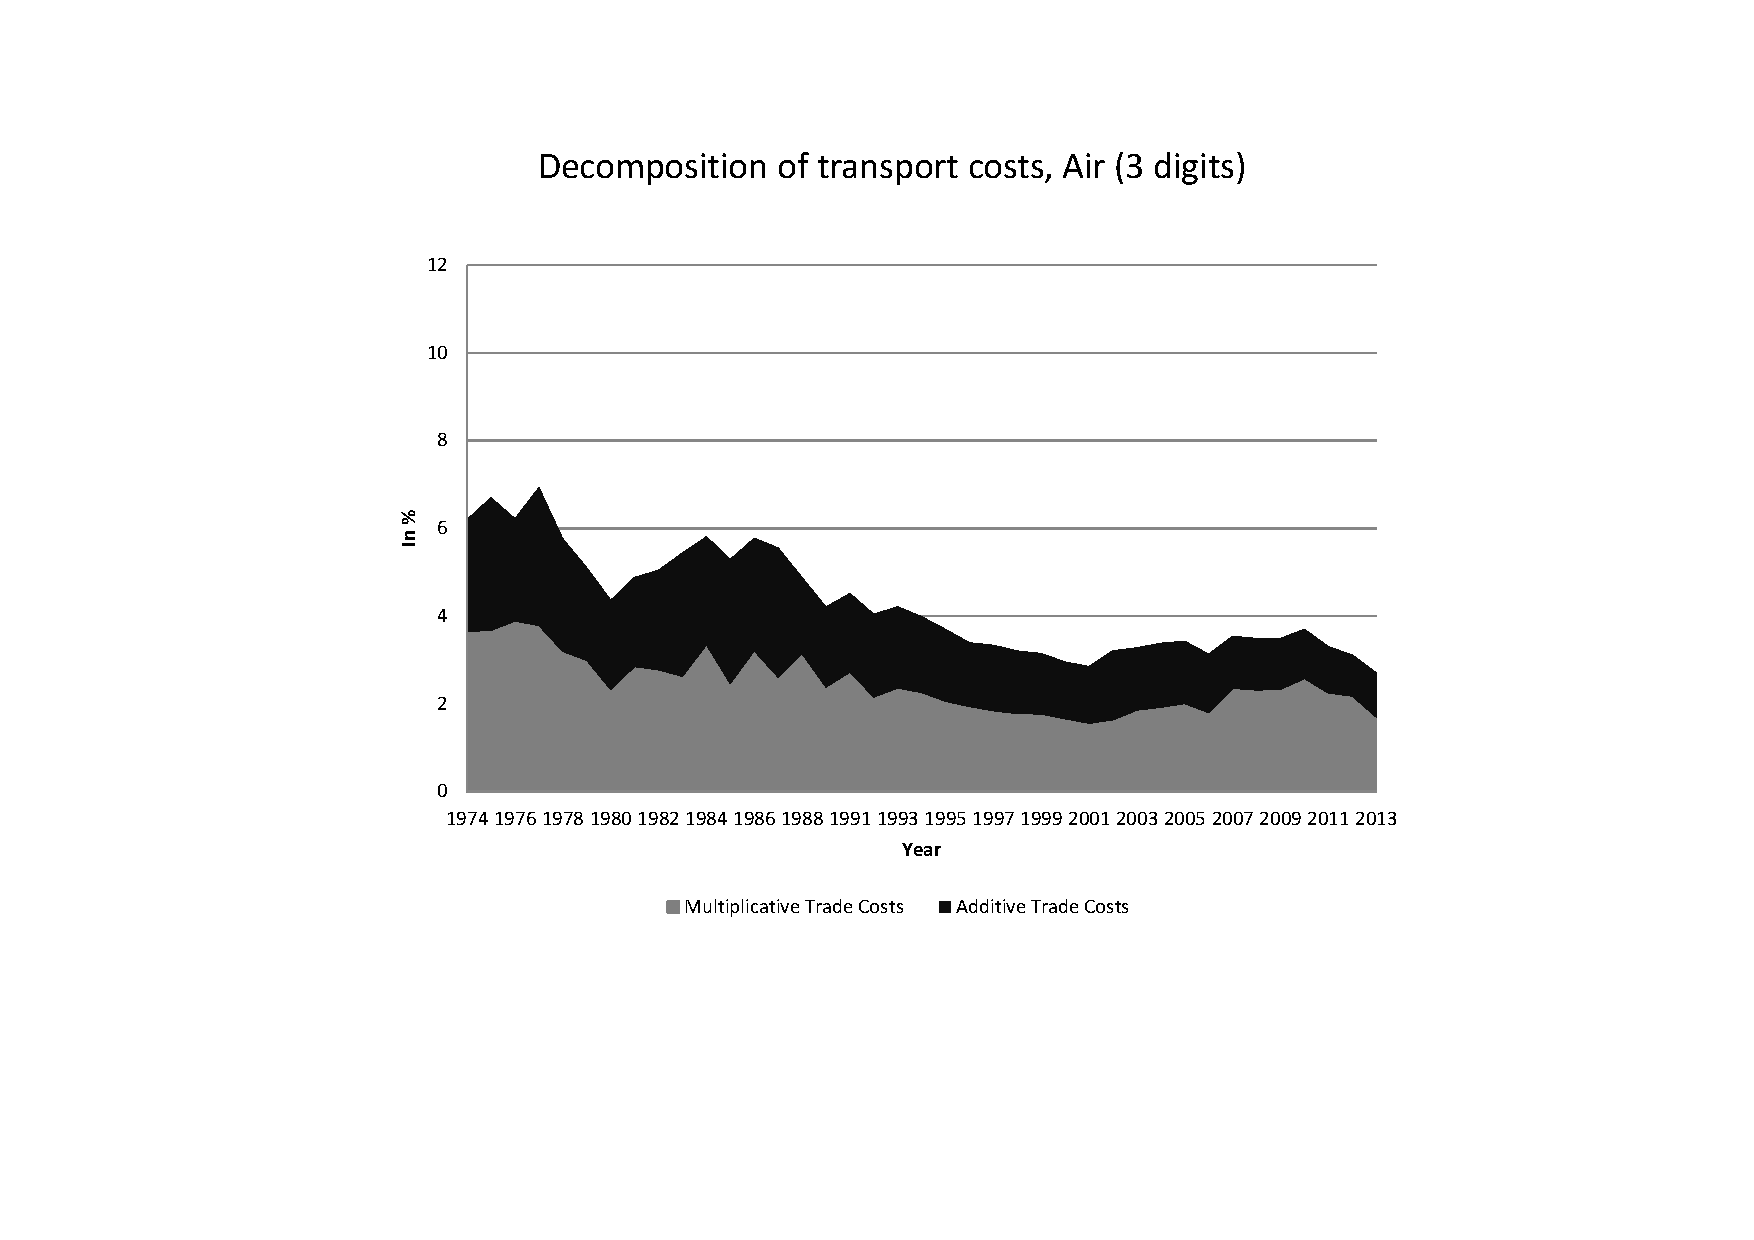
\includegraphics[width=3in, height=2.5in]{Fig2a_decompTC_air_3d.pdf}
& 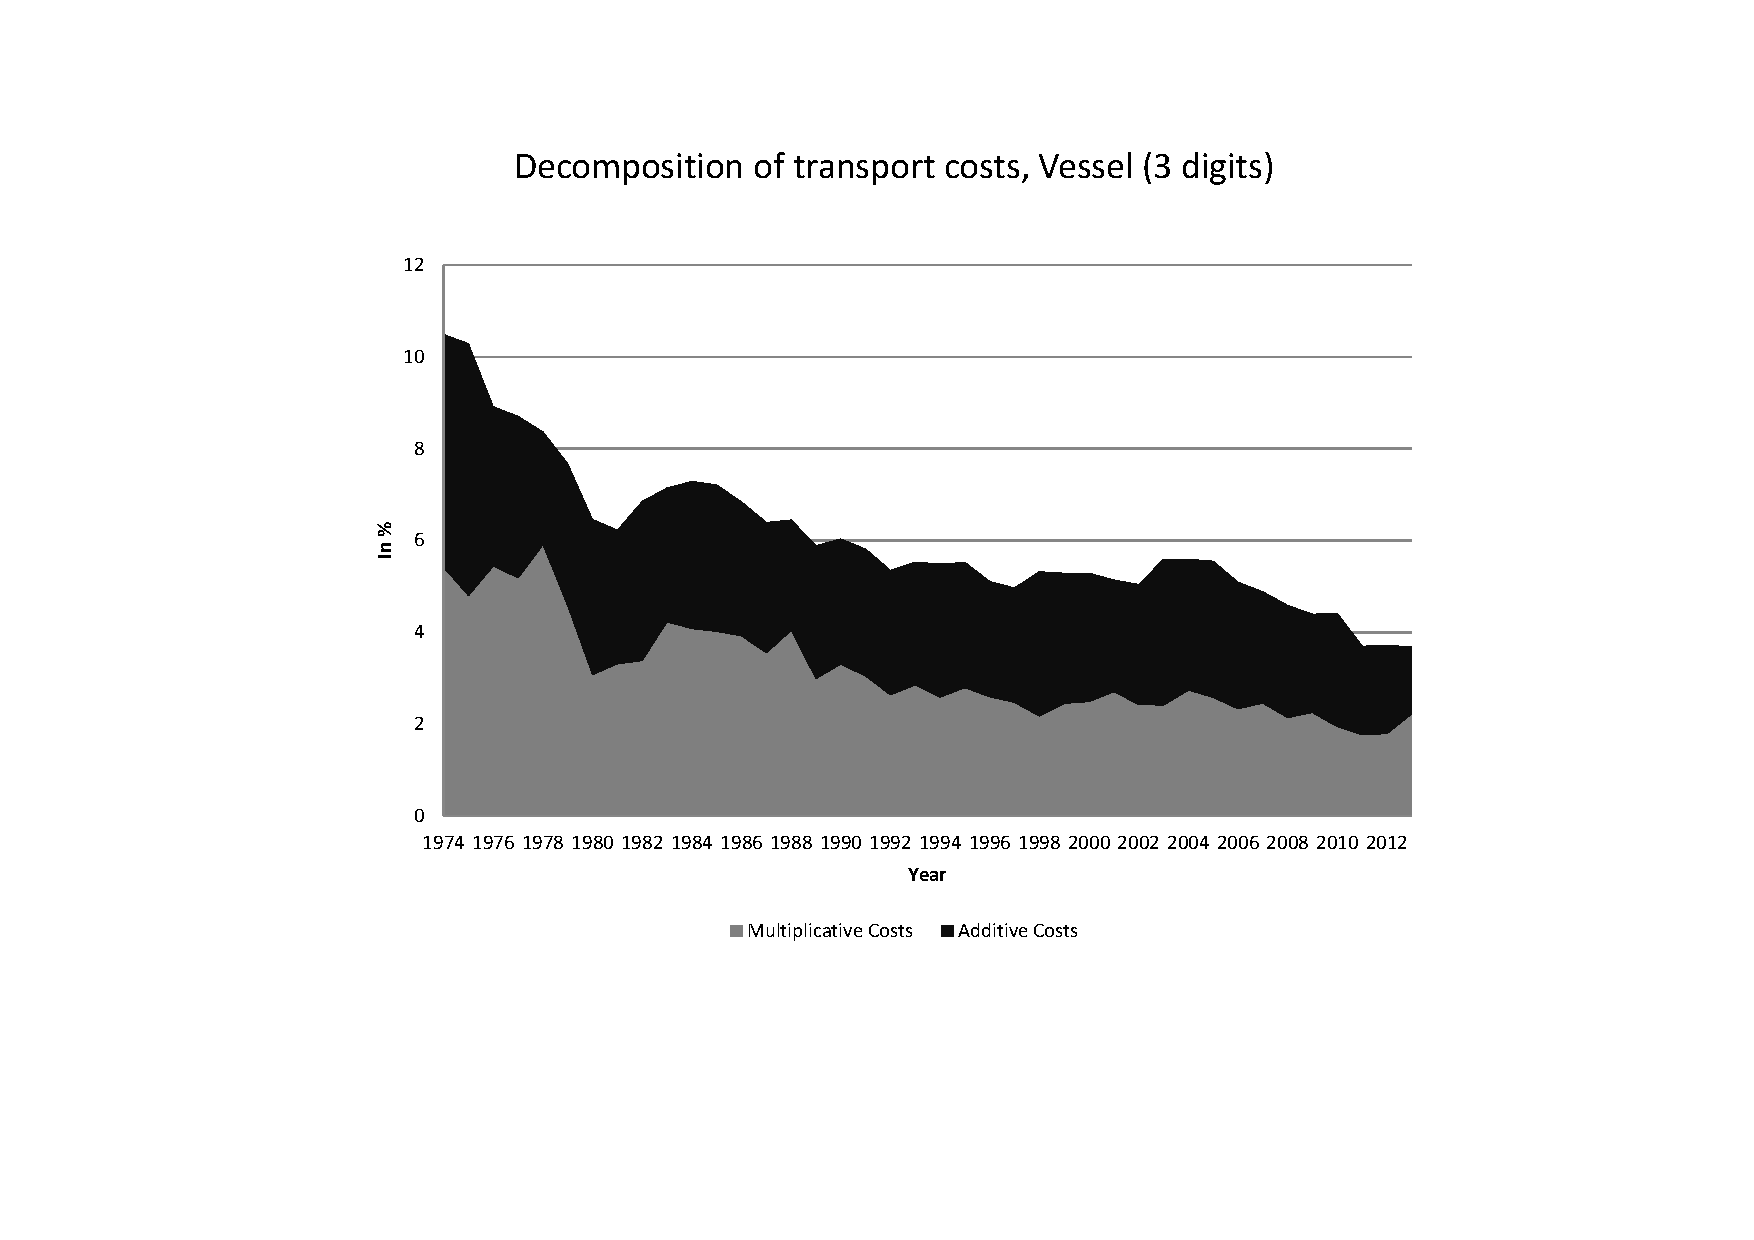
\includegraphics[width=3in,height=2.5in]{Fig2b_decompTC_vessel_3d.pdf} \\
\end{tabular}
\end{center}
\end{figure}

%\textbf{je ne comprends pas les chiffres mis dans le commentaire en 1974, par rapport aux graphiques.}
%JH: Voir Tableaux 4 et 5, années et modes de transport correspondants. Ils correspondent à la mesure "Iceberg alone", parce que cela semblait permettre une comparaison plus directe avec Hummels. Bref, à discuter.

As reported on Figure \ref{fig:decomp_TC_3d}, total transport costs have regularly declined over time, by an order of magnitude of 3 percentage points in air shipping and 5 percentage points in ocean shipping (basically, divided by 2 in both cases). At this point though, we postpone this discussion about the downward trend for transport costs for Section \ref{sec:results_trends}, to focus on the importance of the additive component. In both transport modes, the additive component appears of sizeable importance all over the period, as the share of additive costs remains roughly constant over time. These results thus suggest that additive costs are neither negligible in magnitude nor an erratic phenomenon. By contrast, they represent an sizeable and structural dimension of international transport costs. Further, one side result of our work is to provide quantitative estimates for the values of both additive and ad-valorem transport costs,which can be very useful for the related more theoretical papers, which need to calibrate their models.\medskip

Our estimation results about the size of additive transport costs can be compared to \citet{Irrazabal_2015}, which constitute the most recent evidence on this question. Based on Norwegian trade data for 2004, \citet{Irrazabal_2015} estimate that the ratio of additive to ad-valorem trade costs amounts to 14\% of the export price, ie $\frac{t/\tau}{\widetilde{p}}=14\%$ expressed in our terminology. One important difference with respect to their work is that we can provide separate estimates for each cost component (additive and ad-valorem). From this, we can rebuilt the ratio in similar terms to them -- allowing us to gain in generality in this respect. Making use of our estimates for 2004, we thus obtain a ratio $\frac{t}{\tau\widetilde{p}}=2.8\%$ in ocean shipping, 1.8\% in air transport. This may sound surprisingly low, in contrast to the 14\% obtained by \citet{Irrazabal_2015}. This can be accounted for by recalling the difference in the type of dataset - hence, of costs, embraced in each case. While the database of \citet{Irrazabal_2015} allows to study trade costs in general, our database covers a subset made of the monetary international transport costs (as we start from the gap between the import and the export prices). From \citet{anderson_wincoop_jel}, we can infer that monetary transport costs approximatively represent 15\% of total trade costs.\footnote{\citet{anderson_wincoop_jel} estimate that monetary transport costs represent a 11\% markup over production costs, and that total international trade costs represent 74\%, so transport costs amount to 11/74= 15\% of total trade costs.} Plugging this into \citet{Irrazabal_2015} results, allows to deduce a ratio $t/\tau$ of international transport costs equal to 2.1\% ($0.15\times 0.14$), which is in line with our own results. This makes us confident in our quantitative assessment of the size of the additive component in international transport costs. In the next section, we analyze their importance through another angle based on quality-of-fit diagnostic tests.




\subsection{Assessing the importance of additive transport costs}

In this section, we explore the performances of each type of model (with and without additive costs) in fitting the observed cif-fas prices gap, in order to deliver a more systematic diagnosis about the importance of additive costs. To do so, we rely on several standard measures of fit. The first indicator is through comparing $R^{2}$. However, its use is far from being straightforward when evaluating non-linear estimates.\footnote{$R^2$ is based on the underlying assumption that the adjusted model is a linear one. In a non-linear context, $R^2$ is strictly speaking inappropriate. However, if the error distribution is approximately normal, a standard metric like $R^2$ remains informative on the quality of adjustment.} This drives us to complement the goodness of fit diagnosis with three alternative measures. We provide the Standard Error of Regression (SER), which represents the average distance that the observed values fall from the regression line. The smaller the SER value, the better the quality of fit, as it indicates that the observations are closer to the fitted line. We also report the log-likelihood function, and two measures derived, the Akaike Information Criterion (AIC) and the log-likelihood (LL) ratio test. A decrease in the log-likelihood function points to a better quality-of-fit. However, the likelihood function systematically decreases with the number of parameters included; the AIC criterion allows for correcting this overfitting by including a penalty in the computation of the statistic.\footnote{Precisely, the AIC stat is equal to $2 \times \textrm{number of parameters} - 2 \times \textrm{Likelihood} $, the number of parameters being given by the number of restrictions.} The preferred model is the one with the minimum AIC value. Finally, the log-likelihood ratio test statistic compares systematically the likelihood of the Unrestricted model (\emph{UR}, including the additive term, i.e. Equation (\ref{eq:model_IetA})) and the Restricted one (\emph{R}, i.e. Equation (\ref{eq:model_nlI})). The null tested is that the two models are statistically equivalent. Results are reported in Tables \ref{tab:good_fit_air} and \ref{tab:good_fit_vessel}, for Air and Vessel respectively, at the 3-digit level.



\begin{table}[htbp]
  \centering
  \caption{Air: Measures of Goodness-of-fit (3 digits)}
  \footnotesize{
\begin{center}
    \begin{tabular}{l|cccccc|c}
    \hline \hline
    Year  & 1974  & 1980  & 1990  & 2000  & \multicolumn{1}{c}{2010} & \multicolumn{1}{c}{2013} & Mean stat \\ \hline
    \multicolumn{8}{l}{\bf{$R^2$} }\\ \hline
    Model (A)& 0.30  & 0.27  & 0.25  & 0.32  & \multicolumn{1}{c}{0.42} & \multicolumn{1}{c}{0.34} & 0.31 \\
    Model (B) & 0.59  & 0.65  & 0.63  & 0.64  & \multicolumn{1}{c}{0.51} & \multicolumn{1}{c}{0.46} & 0.60 \\ \hline
    \multicolumn{8}{l}{\textbf{SER}  }  \\ \hline
     Model (A) & 0.79  & 0.86  & 0.81  & 0.84  & \multicolumn{1}{c}{0.86} & \multicolumn{1}{c}{0.92} & 0.85 \\
    Model (B) & 0.67  & 0.71  & 0.67  & 0.70  & \multicolumn{1}{c}{0.79} & \multicolumn{1}{c}{0.85} & 0.73 \\ \hline
   \multicolumn{8}{l}{\textbf{AIC criteria}}  \\ \hline
    Model (A) & 35675.0 & 41171.0 & 60715.6 & 87492.6 & \multicolumn{1}{c}{102297.7} & \multicolumn{1}{c}{88191.9} & 70498.1 \\
    Model (B)  & 31387.3 & 35738.4 & 52098.9 & 74954.9 & \multicolumn{1}{c}{95887.1} & \multicolumn{1}{c}{80873.7} & 62285.0 \\ \hline
    \multicolumn{8}{l}{\textbf{Log-likelihood}} \\ \hline
    Model (A) & -17530.5 & -20253.5 & -29977.8 & -43341.3 & \multicolumn{1}{c}{-50746.8} & \multicolumn{1}{c}{-43692.9} & -34888.6 \\
    Model (B) & -15125.6 & -17263.2 & -25393.5 & -36788.4 & \multicolumn{1}{c}{-47277.5} & \multicolumn{1}{c}{-39751.9} & -30508.3 \\
    LL ratio & 4809.7 & 5980.6 & 9168.7 & 13105.7 & \multicolumn{1}{c}{6938.6} & \multicolumn{1}{c}{7882.1} & 8760.69 \\
    nb of restrictions & 355   & 369   & 393   & 426   & \multicolumn{1}{c}{426} & \multicolumn{1}{c}{427} & 402 \\
    p-value & 0.00 & 0.00 & 0.00 & 0.00 & \multicolumn{1}{c}{0.00} & \multicolumn{1}{c}{0.00} & 0.00 \\
    \hline \hline
 \end{tabular}%
    \end{center}}
  \label{tab:good_fit_air}%
 \parbox[l]{12cm}{\tiny{Notes: Model (A) = with only ad-valorem transport costs. Model (B) = with additive \& ad-valorem transport costs. SER = Standard Error of regression; AIC = Akaike Information Criterion. $R^{2}$ between the log of predicted ratio and the log of the observed ratio. For the LL ratio test, the number of restrictions is equal to the number of parameters estimated, i.e., the number of partner countries plus the number of products. The mean statistics calculated as the average value over all years. }}
\end{table}%

\begin{table}[htbp]
  \centering
  \caption{Vessel: Measures of Goodness-of-fit (3 digits)}
    \footnotesize{
\begin{center}
\begin{tabular}{l|cccccc|c}
\hline \hline
Year  & \multicolumn{1}{c}{1974} & \multicolumn{1}{c}{1980} & \multicolumn{1}{c}{1990} & \multicolumn{1}{c}{2000} & 2010  & \multicolumn{1}{c}{2013} & Mean stat \\ \hline
\multicolumn{8}{l}{\bf{$R^2$} }\\ \hline
Model (A)& \multicolumn{1}{c}{0.45} & \multicolumn{1}{c}{0.42} & \multicolumn{1}{c}{0.46} & \multicolumn{1}{c}{0.40} & 0.35 & \multicolumn{1}{c}{0.34} & 0.39 \\
  Model (B) & \multicolumn{1}{c}{0.61} & \multicolumn{1}{c}{0.58} & \multicolumn{1}{c}{0.59} & \multicolumn{1}{c}{0.57} & 0.49 & \multicolumn{1}{c}{0.46} & 0.56 \\ \hline
\multicolumn{8}{l}{\textbf{SER}  }  \\ \hline
    Model (A) & \multicolumn{1}{c}{0.58} & \multicolumn{1}{c}{0.62} & \multicolumn{1}{c}{0.59} & \multicolumn{1}{c}{0.65} & 0.74  & \multicolumn{1}{c}{0.76} & 0.66 \\
    Model (B) & \multicolumn{1}{c}{0.48} & \multicolumn{1}{c}{0.53} & \multicolumn{1}{c}{0.51} & \multicolumn{1}{c}{0.55} & 0.66  & \multicolumn{1}{c}{0.68} & 0.57 \\ \hline
   \multicolumn{8}{l}{\textbf{AIC criteria}}  \\ \hline
   Model (A) & \multicolumn{1}{c}{33328.8} & \multicolumn{1}{c}{33010.3} & \multicolumn{1}{c}{51142.6} & \multicolumn{1}{c}{71365.9} & 84789.9 & \multicolumn{1}{c}{88191.9} & 57848.6 \\
   Model (B) & \multicolumn{1}{c}{27331.5} & \multicolumn{1}{c}{28067.3} & \multicolumn{1}{c}{43664.7} & \multicolumn{1}{c}{60475.9} & 76161.3 & \multicolumn{1}{c}{80873.7} & 49682.3 \\ \hline
    \multicolumn{8}{l}{\textbf{Log-likelihood}} \\ \hline
    Model (A) & \multicolumn{1}{c}{-16287.4} & \multicolumn{1}{c}{-16129.1} & \multicolumn{1}{c}{-25169.3} & \multicolumn{1}{c}{-35263.9} & -41998.9 & \multicolumn{1}{c}{-43692.9} & -28534.3 \\
    Model (B) & \multicolumn{1}{c}{-12985.8} & \multicolumn{1}{c}{-13353.7} & \multicolumn{1}{c}{-21171.4} & \multicolumn{1}{c}{-29491.0} & -37418.7 & \multicolumn{1}{c}{-39751.9} & -24151.3 \\
    LL ratio & \multicolumn{1}{c}{6603.28} & \multicolumn{1}{c}{5550.96} & \multicolumn{1}{c}{7995.88} & \multicolumn{1}{c}{11545.98} & 9160.56 & \multicolumn{1}{c}{7882.15} & 8766.0 \\
    nb of restrictions & \multicolumn{1}{c}{393} & \multicolumn{1}{c}{395} & \multicolumn{1}{c}{411} & \multicolumn{1}{c}{436} & 424   & \multicolumn{1}{c}{427} & 417 \\
    p-value& \multicolumn{1}{c}{0.00} & \multicolumn{1}{c}{0.00} & \multicolumn{1}{c}{0.00} & \multicolumn{1}{c}{0.00} & 0.00  & \multicolumn{1}{c}{0.00} & 0.00 \\
    \hline \hline
    \end{tabular}%
    \end{center}}
  \label{tab:good_fit_vessel}%
  \parbox[l]{12cm}{\tiny{Notes: Model (A) = with only ad-valorem transport costs. Model (B) = with additive \& ad-valorem transport costs. SER = Standard Error of regression; AIC = Akaike Information Criterion. $R^{2}$ between the log of predicted ratio and the log of the observed ratio. For the LL ratio test, the number of restrictions is equal to the number of parameters estimated, i.e., the number of partner countries plus the number of products. The mean statistics calculated as the average value over all years. }}
\end{table}%


Tables \ref{tab:good_fit_air} and \ref{tab:good_fit_vessel} lead to the same conclusion: The inclusion of the additive term leads to an improvement of the quality of fit, whatever the considered criterion or the transport mode. On average over the whole period, the $R^{2}$ doubles when per-kg costs are included for Air, and increases by 50\% for Vessel. Similar qualitative conclusions arise from the comparisons of the standard errors of the regression (SER). Regarding the other criteria, improvements allowed by the inclusion of the additive term are roughly of the same extent across transport modes. Both AIC and Log-Likelihood statistics decrease with the inclusion of the additive term, and the log-likelihood test unambiguously rejects the null of statistical equivalence of the two models. These results holds whatever the considered year.\smallskip


For comparison purposes, we provide a similar goodness-of-fit exercise at the 4-digit product level (4-digits), reported in in Appendix \ref{app:4digit}, Tables \ref{tab:good_fit_air_rob} and \ref{tab:good_fit_ves_rob}. If anything, the quality of fit appears slightly higher when estimations are based on the 4-digit classification. This is especially true for the model restricting transport cost to their ad-valorem dimension, whatever the transport mode considered. When the additive part is taken into account however, the difference in goodness of fit between the 3- and the 4-digit classification level becomes very small, whatever the considered criterion. In other words, if using a more disaggregated classification unsurprisingly adds some statistical precision, this is not to an extent that would disqualify the use of slightly more aggregated data. Further, the same conclusion established at the 3-digit level regarding the significant role of the additive component in fitting international transport costs emerges at the 4-digit level.



\section{Transport Costs time trends: The role of the additive component}\label{sec:results_trends}
\subsection{Estimation strategy}
In this section, we investigate the role of the additive component in total transport costs in a historical perspective.
As a first step, we come back to Figure \ref{fig:decomp_TC_3d}, that displays the respective shares of additive and iceberg components in transport costs over time by transport mode. Considering the trend in total transport costs (the upper line in Figure \ref{fig:decomp_TC_3d}), both air and vessel shipping exhibit a downward trend in overall transport costs since 1974, by -2.1\% per year for mean air transport costs and -2.0\% per year for mean ocean transport costs, implying a 50\% decrease in Air and a 60\% decrease in Vessel over the period.\footnote{One may be puzzled for by the high magnitude of estimates for the beginning of the period (until 1980 approximately) for ocean transport. \citet{hummels2007} finds similar outcomes on tramp prices indexes, and suggests the oil shock as a likely culprit, in a context where technological progress was quicker in aviation than in vessel, allowing a better dampening of oil shocks on air freight rates. In a related manner, one may worry that the strong decrease in transport costs documented in Figure \ref{fig:decomp_TC_3d} springs from high oil-shock related transport costs in 1974. However, computing the time trends from 1980 does not dramatically change the picture. The yearly trend from 1980 is -2\% for mean air transport costs and -1.6\% for mean vessel transport costs. We thus choose to exploit the whole time dimension of our database by taking 1974 as starting date of our time trend analysis.} On US data, \citet{Hummels_1999} obtains that overall transport cost declined from 6 \% to 4 \% of the import value between 1974 and 1996. For the same years, we obtain a total decrease from 6.9 to 4.2\% in terms of the export price, on average for air shipping, and from 9.8\% to 4.8\% for ocean shipping. Overall, our results display trends that are close to those reported by \citet{Hummels_1999}, with a magnitude of transport costs that appears higher in ocean shipping than for air transport over the period.

Before making any definite statement about this though, it is worth emphasizing that the time trend of international transport costs depends on both \textit{i)} the evolution of per product and per partner ``ceteris paribus'' transport costs and \textit{ii)} the evolution of the composition of trade. Total transport costs may thus have decreased over time because the share of neighbor countries in total US trade or the share of goods cheaper to transport has increased (explanation \textit{ii)}), independently of any change in transport costs \textit{per se}. As emphasized by \citet{Hummels_1999} or \cite{hummels2007}, it is hence necessary to eliminate the composition effects of trade flows to isolate the evolution of ``ceteris paribus'' international transport costs, i.e. per product- and per partner- transport costs.

If we share this view with \cite{hummels2007}, we adopt a different strategy for eliminating composition effects, which builds upon our first-stage results.\footnote{See Appendix \ref{app:compare_Hummels} for a detailed comparison of Hummel's (2007) methodology and ours.} Estimation driven in Section \ref{sec:results_decomposition} indeed provides us with the additive and ad-valorem measures of international transport costs (Equation (\ref{eq:model_IetA})), that vary over time, product and origin country. Starting from these values, we extract the ``ceteris paribus'' transport cost measure, for each additive and multiplicative cost component (by transport mode) by the mean of a time fixed effect (see details below). For each cost component (additive and ad-valorem), comparing the unfitted measure and the fitted measure (composition effects excluded) allows to characterize if the decrease observed over the period is due to trade composition effects (for instance, changes in the country partners, in the type/ quality of products traded), or if it is the ``ceteris paribus'' costs (for instance, insurance or handling costs) that have reduced over time. We conduct the same analysis on a overall transport costs measure, built by agglomerating the two estimated components (additive and iceberg) in a unified measure of transport costs.\footnote{Note that the ``unfitted'' total transport costs are virtually the same as those reported in Figure \ref{fig:decomp_TC_3d}, but reported from another perspective (basis 100 in year 1974).}

\subsection{Empirical specification}
Our strategy to eliminate the composition effects obeys the following rationale. As explained above, we start from the values of each additive and ad-valorem transport cost measure estimated in Section \ref{sec:results_decomposition}. We extract the changes over time in the ``ceteris paribus'' transport cost dimension by assuming a composition of trade flows by country partner and product that is constant throughout the period, and equal to the one observed in 1974. One advantage of this method is to yield measures of transport costs (fitted and unfitted) that are easily comparable between transport modes and transport cost components.

This can be described as a two-stage process. First, for each transport costs component (additive/multiplicative), we decompose the estimated measure in the three product/country/time dimensions, using fixed effects. For the estimated ad-valorem component, we thus estimate the following equation:
\begin{eqnarray}
\ln(\widehat{\tau}_{ikt})&=&\delta +\underbrace{\sum_{i \neq \text{ARG}}\alpha_i.\mathbb{1}_i}_{(a)} + \underbrace{\sum_{s(k)\neq \text{011}}\beta_{s(k)}.\mathbb{1}_{s(k)}}_{(b)} + \underbrace{\sum_{t \neq 1974}\gamma_t.\mathbb{1}_t}_{(c)}+\epsilon_{ikt} \label{eq:compeffects_mult}
\end{eqnarray}

\noindent where $\mathbb{1}_i$ and $\mathbb{1}_{s(k)}$ represent country- and sector- fixed effects.\footnote{Throughout the exercise, we consider Argentina, the sector 011 and the first year of our dataset 1974, as references for the country-, product and -year dummies.}  Equation (\ref{eq:compeffects_mult}) is estimated using OLS, with a weighting scheme based on the value of each flow in the total value of flows the considered year. As for the additive component, given that the sector fixed effect and the country fixed effect are additive rather than multiplicative by construction, we estimate the following equation using non-linear least squares (using the same weighting scheme):\footnote{For sake of notational simplicity, we do not distinguish the coefficients associated to the fixed effects between Equations (\ref{eq:compeffects_mult}) and (\ref{eq:compeffects_add}), even if they are specific to the type of transport costs considered (e.g., the series of $\gamma_t$ differs from one estimation to the other). Note that we impose the same weighting scheme as for the OLS regression (based on the relative value of the flow).}
%, based on the additive cost series $\widehat{t}_{ikt}$ previously obtained:
\begin{eqnarray}
\ln(\widehat{t}_{ikt})&=&\ln\left( \delta + \underbrace{\sum_{i \neq \text{ARG}}  \alpha_i.\mathbb{1}_i}_{(a)}+\underbrace{\sum_{s(k)}\beta_{s(k)}.\mathbb{1}_{s(k)}}_{(b)}\right) + \underbrace{\sum_{t \neq 1974}\gamma_t.\mathbb{1}_t}_{(c)}+\epsilon_{ikt} \label{eq:compeffects_add}
\end{eqnarray}
As displayed in Equations (\ref{eq:compeffects_mult}) and (\ref{eq:compeffects_add}), the objective is to decompose the estimated transport cost component in three components: The country dimension (Term (a)), the product dimension (Term (b)) and the ``ceteris paribus'' transport costs time trend (Term (c)). Notice that Equations (\ref{eq:compeffects_mult}) and (\ref{eq:compeffects_add}) preserve our specification of the ad-valorem and additive costs of Equations (\ref{eq:ad-valorem}) and (\ref{eq:add}), as we consider that the iceberg cost is the product of the country of origin and the good dimension, while the additive cost is the sum of the two dimensions. Both equations are estimated by transport mode.

In this exercise, we are interested in isolating the change in the time dimension of the each transport cost component. This constitutes our second stage. As for the ad-valorem component defined in $[1;+\infty]$, from the estimation of Equation (\ref{eq:compeffects_mult}), we built the variable $\Gamma^{adv}_t$, for each year $t\geq 1974$, according to:\footnote{See details in Appendix \ref{app:comp-effects}.}
\begin{equation}
\Gamma^{adv}_t = 100.\frac {\bar{\tau}_{1974}.\exp(\gamma_t)-1} {\bar{\tau}_{1974}-1} \label{eq:comp_effects_adv}
\end{equation}

\noindent with $\bar{\tau}_{1974} = \exp(\delta +\sum_i \alpha_i +\sum_s \beta_s)$ the mean ad-valorem transport cost in 1974. In plain words, we measure how these costs have changed over time by blocking the composition of trade flows by product and country partners to the one observed in 1974 (the beginning of our sample).

As for the additive cost defined in $[0;+\infty]$, we built the variable $\Gamma^{add}_t$, the reference year being 1974 (ie, with $\gamma_{1974}=0$) according to:
\begin{equation}
\Gamma^{add}_t = 100.\exp(\gamma_t) \label{eq:comp_effects_add}
\end{equation}

\noindent As a result, the two series (for $\Gamma^{adv}_t$ and $\Gamma^{add}_t$) have a straightforward interpretation in percentage changes from the initial value of 100 for $t=1974$.

Last, we rebuild a measure of total transport costs as the sum of the two components (additive and iceberg), on both the unfitted measures  and the ``ceteris paribus'' estimated transport costs (composition effects excluded). Details are reported in Appendix \ref{app:comp-effects}.


\subsection{Characterizing the time trends in transport costs}
Figure \ref{fig:totalTC_compeffects_excl} reports the results.\footnote{Figure \ref{fig:totalTC_compeffects_excl} reports the results, all types of goods included. In Appendix \ref{app:comp-effects}, we report the results at a more disaggregated level, distinguishing between primary and manufacturing goods.} Panels (a), (b) and (c), we report the time changes of the ad-valorem costs, the additive costs and the total costs respectively, for Air transport (starting from the reference value 100 in 1974). Panels (d), (e) and (f) report the results for Vessel. In each panel, we report the evolution of transport costs for both the unfitted (plain blue line) and the fitted (dotted red line) measures.


\begin{figure}[htbp]
\caption{Transport costs (with and without composition effects)}
\label{fig:totalTC_compeffects_excl}
\begin{center}
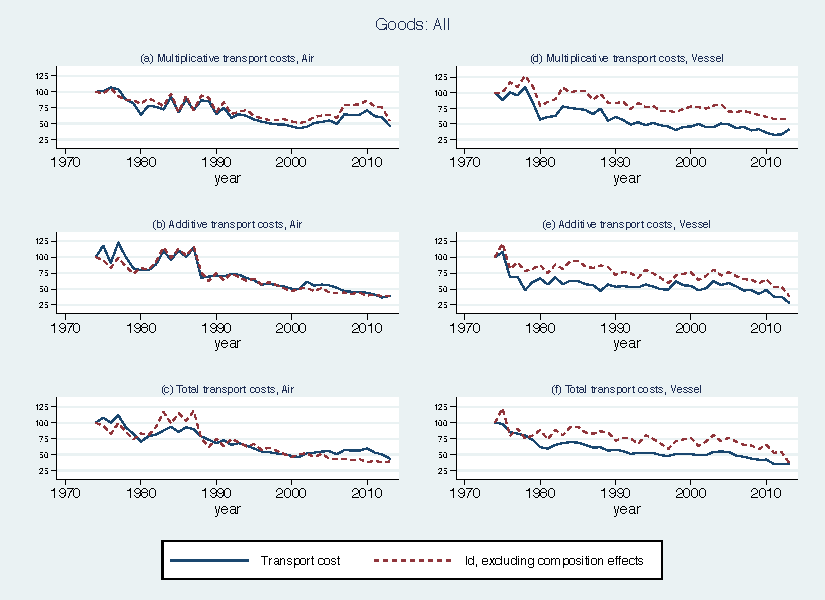
\includegraphics[height=4in]
{graph_composition_all.pdf}
\end{center}
\end{figure}

Three main results emerge from Figure \ref{fig:totalTC_compeffects_excl}. First, in accordance with Figure \ref{fig:decomp_TC_3d}, we find that international transport costs have substantially decreased over the period, and in both transport modes. International transport costs were reduced by 50\% between 1974 and 2013 in air shipping, and by 60\% in maritime shipping. This stands in line with the related literature (see \citealp{Hummels_1999}, \citealp{Lafourcade_Thisse}). Second, and as discussed in Section \ref{sec:results_decomposition}, the magnitude of the decrease is roughly of same order both the ad-valorem and the additive components. Third, and most importantly, we find that composition effects do not play a major role in accounting for the time trend of overall transport costs. Inspecting the panels of Figure \ref{fig:totalTC_compeffects_excl}, we do not find much evidence of a substantial difference between the unfitted transport costs measure and the ``ceteris paribus'' transport costs. This is particularly true in Air transport, for both the additive and ad-valorem components (Figure \ref{fig:totalTC_compeffects_excl}, panels (a) to (c)). Air transport costs were reduced by 50\% between 1974 and 2013, and this is mainly attributable to a reduction in the ``ceteris paribus'' transport costs. Composition effects are more pronounced in vessel transport. Considering the raw series, maritime transport costs have decreased by 60\% over the period, which can be decomposed in a 50\% decrease in transport costs \textit{per se}, and a 10\% reduction that comes from composition effects, in particular for the multiplicative component (panel (d)).\smallskip

\subsection{Time trends in transport costs and the modeling of the additive component}

This last result stands in sharp contrast with \citet{hummels2007}, which obtains that the ``ceteris paribus'' transport costs had decreased more than the unfitted ones (over 1974-2004), suggesting an important role to composition effects. If anything, we find the opposite result here. This drives us to investigate this difference of result further. As we explain in more details in Appendix \ref{app:comp-effects}, our empirical strategy differs from \cite{hummels2007} in one main dimension. Our characterization of the time trends in transport costs starts from our estimates of both the additive and the ad-valorem components (obtained in Section \ref{sec:results_decomposition}), as well as for the overall transport cost (rather than the actual cif-fas price gap). As direct consequence, our methodology lets the ratio between the additive and the ad-valorem components of transport costs vary over the three time-product-partner country dimensions. %By contrast, \cite{hummels2007} does not take into account the changes in the additive transport cost component, attributing this to a change in the composition of the bundle over time (per country-commodity).
This turns out to be of primary importance in the disentangling in the time trend of transport costs, between what comes from the trade composition effects and what comes from changes in the ``ceteris paribus'' transport cost dimension, as we show below. \footnote{As discussed in Appendix \ref{app:comp-effects}, our methodology also differs from  \citet{hummels2007} with respect to the weighting scheme used to obtain the evolution of the ``ceteris paribus'' transport costs over time. Robustness analysis to this point is driven in Section \ref{sec:robustness}.} To establish this point clearly, we replicate the method adopted by \cite{hummels2007} exposed above on our database (which is the same as his until 2004). The results are reported in Figure \ref{fig:comp_effects_as_in_Hummels}. The dotted line labeled ``expenditure/import value'' represents the unfitted measure of transport costs ($TC_t$ in the above terminology) and the plain line labeled ``fitted ad-valorem rate'' is the measure of transport costs composition effects excluded ($\widehat{TC}_t$).

\begin{figure}[htbp]
\caption{Characterizing the time trends: Applying Hummel's (2007) method }
\label{fig:comp_effects_as_in_Hummels}
\begin{center}
\begin{tabular}{cc}
{\small (a) Ad-valorem Air Freight} & {\small (b) Ad-valorem Vessel Freight}\\
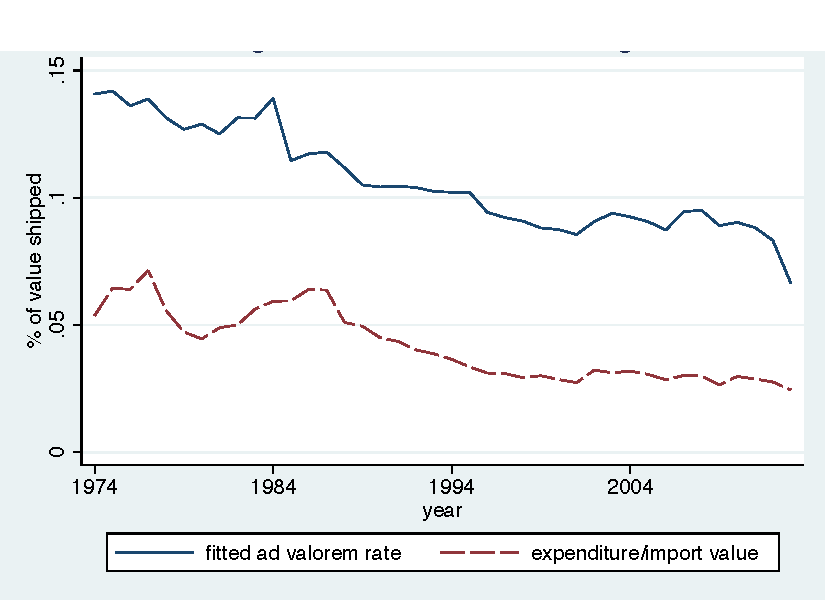
\includegraphics[width=3in, height=2.5in]{figure5_comme_hummels_air.pdf}
& 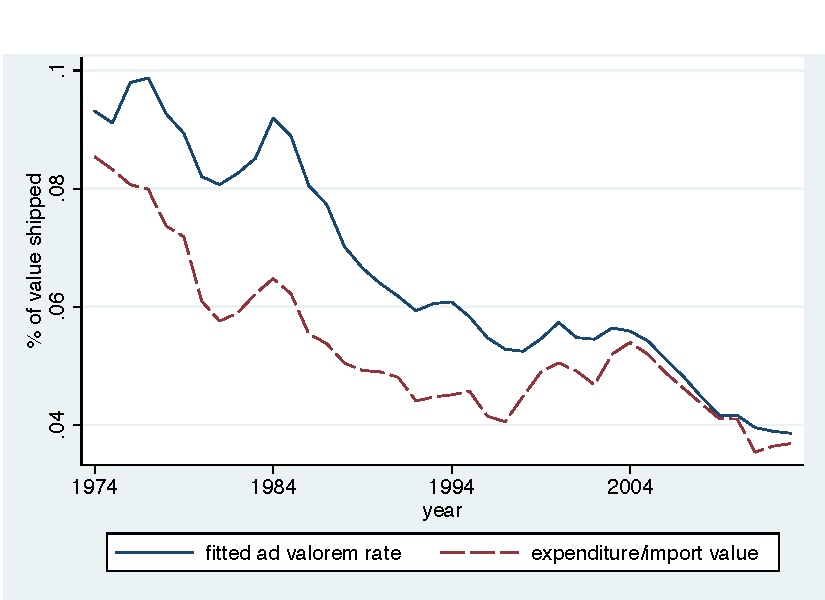
\includegraphics[width=3in,height=2.5in]{figure6_comme_hummels_ocean.pdf} \\
\end{tabular}
\end{center}
\end{figure}

These results stand in sharp contrast with the ones obtained with our methodology and reported in Figure \ref{fig:totalTC_compeffects_excl}. Applying \citeh{hummels2007} method, we obtain that the composition effects tend to partially offset the decrease in transport costs in both air and vessel shipping (as the downward trend is of higher magnitude for the fitted than the unfitted rate, especially for Vessel).\footnote{Unsurprisingly, this stands in accordance with \citeh{hummels2007} results, see his Figures 5 (for Air) and 6 (for Vessel)} This result is overturned when we allow for more flexibility in the role of the additive component, as depicted in Figure \ref{fig:totalTC_compeffects_excl}. Assuming a varying share of the additive component over time, product and country partner indeed modifies the decomposition of the trend reduction of transport costs between the one attributable to trade composition effects and the reduction in the ``ceteris paribus'' transport costs. In both air and vessel transports, we thus find that this last dimension is the main driver of the reduction of international transport costs observed over time, in particular in vessel transport. Complementing the findings of Section \ref{sec:results_decomposition}, these results point out the importance of integrating the additive dimension of international transport costs, here in view of characterizing their time trends.



%\section{Robustness checks \label{sec:robustness}}

%\subsection{Measuring transport costs components: Robustness to the separability assumption}


%Ie, estimate


%$$\log(\frac{p_{ik}}{\widetilde{p}_{ik}} -1)= \log(\tau_{is} -1+ \frac{t_{is}}{\widetilde{p}_{ik}})+ \exp(\epsilon_{ik})$$

%To do on 100 products ($s$), 50 countries (the most important?)

\section{Time trends in transport costs: Robustness to the weighting scheme \label{sec:robustness}}

In this section, we provide a robustness test to the weighting scheme implemented to extract the trade composition effects implemented in Section \ref{sec:results_trends}. When aggregating the trade cost measure over the product/country ($i,k$) dimension, \cite{hummels2007} takes the unweighed average value over the $i,k$ dimension, which implicitly attributes a weight equal to 1 to each flow. We proceed differently, as we weight each flow by its relative value on total trade flows observed in 1974. In this section, our objective is to assess that this difference of treatment is not responsible for the difference of results relative to the role of the trade composition effects, that we rather attribute to the modeling of the additive component.

To this aim, we rebuild the fitted values for each of of our transport cost measures (ad-valorem, additive and overall) applying Hummels' s (2007) weighting scheme (ie, taking the unweighed average value over the $i,k$ dimension), which we then express as indices, with the reference value 100 in 1974. The results are reported in Figure \ref{fig:compeffects_robustness}.

\begin{figure}[htbp]
\caption{Transport cost time trends: Robustness to the weighting scheme}
\label{fig:compeffects_robustness}
\begin{center}
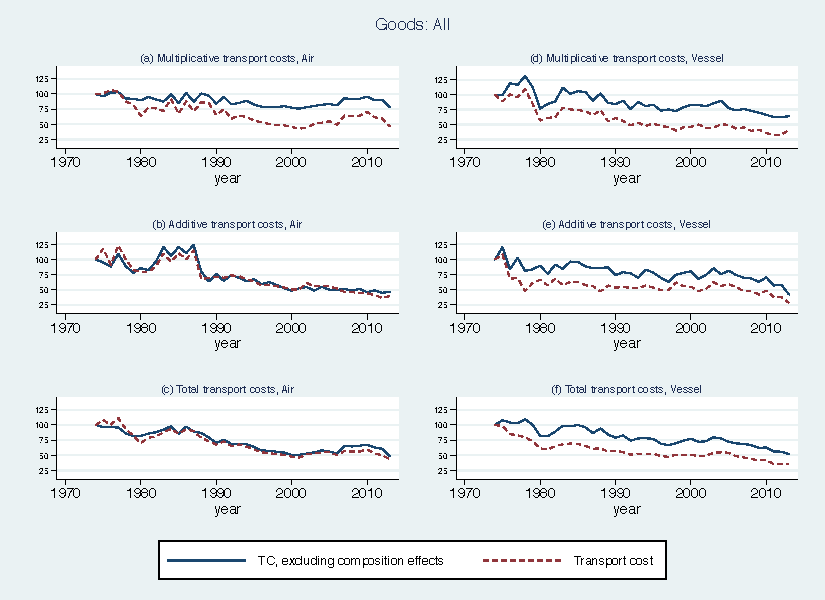
\includegraphics[height=8cm]
{graph_composition_all_np.pdf}
\end{center}
\end{figure}

The comparison of Figure \ref{fig:compeffects_robustness} (applying Hummels's (2007) weighting scheme) and Figure \ref{fig:totalTC_compeffects_excl} (applying our weighing scheme) drives two comments. First, differences do show up, in particular for the multiplicative component of Air transport. This suggests that the weighting scheme is not innocuous in the time trend decomposition exercise. However, Figure \ref{fig:compeffects_robustness} also shows that the composition effects have contributed to strengthen the decrease in the ``ceteris paribus'' transport costs in Air transport (in Figure \ref{fig:compeffects_robustness}, panel (a), overall transport costs have decreased more that the fitted component), in accordance with the conclusions drawn from Figure \ref{fig:totalTC_compeffects_excl}, rather than to partially offset as argued by \cite{hummels2007}. Rather than the weighing scheme, this confirms that the functional form and precisely the modeling of the additive component, turns out to be key in understanding the underlying determinants of the overall transport costs time trends, as we pointed out in Section \ref{sec:results_trends}.

\section{Conclusion \label{sec:conclu}}

This paper empirically studies the magnitude of additive (or per-kg) costs in international transport costs, by exploiting the differences between the import and the export prices. Using SITC 3 and 4- digit cif-fas unit values taken from the US import database over 1974-2013, we estimate the two components of transport costs, by transport mode (air or ocean).  Our results may be summarized in three main findings. First, we provide a quantitative measure of both the additive and the iceberg transport cost. We thus find that additive costs amount to 2.8\% of the export price unit values for ocean shipping, and ad-valorem ones 3.2\%, as mean values over 1974-2013. These values are respectively equal to 1.8 and 2.5\% for air transport. Second, we show that taking additive costs into account improves the fit of the modeling of transport costs. All goodness-of-fit measures point out to this conclusion, which holds for both transport modes and all years considered. Third, we show the importance of integrating the additive component in accounting for the time trend of international transport costs. Allowing for a varying share of additive costs in product/country/time dimension, we obtain that the decrease of international transport costs observed in the data is mostly attributable to a reduction in the \textit{pure} transport costs rather than to trade pattern composition effects. In all three aspects, our results point the importance of the additive component in accounting for international transport costs.

Our results could be extended in two main ways. On the empirical side, one may want to go deeper in the ``structural'' determinants of trade costs, i.e. identify the respective roles of handling costs, insurance and freight at the root of the gap between export and import prices. On the theoretical side, our results can be used to explore the role of additive costs in shaping international trade flows (in an international trade theory perspective) and in affecting the international transmission of business cycles. This is left for further research.



\newpage
\bibliographystyle{essaien}
\bibliography{biblio}


\newpage


\appendix

\section{Data Appendix \label{app:data}}


The Customs value is the value of imports as appraised by the U.S. Customs and Border Protection in accordance with the legal requirements of the Tariff Act of 1930, as amended. This value is generally defined as the price actually paid or payable for merchandise when sold for exportation to the United States, excluding U.S. import duties, freight, insurance, and other charges incurred in bringing the merchandise to the United States. The term ``price actually paid or payable'' means the total payment (whether direct or indirect, and exclusive of any costs, charges, or expenses incurred for transportation, insurance, and related services incident to the international shipment of the merchandise from the country of exportation to the place of importation in the United States) made, or to be made, for imported merchandise by the buyer to, or for the benefit, of the seller. In this respect, the ``custom value'' corresponds to the fas price (``free-alongside'' price) delivered by the seller.

The import charges represent the aggregate cost of all freight, insurance, and other charges (excluding U.S. import duties) incurred in bringing the merchandise from alongside the carrier at the port of exportation in the country of exportation and placing it alongside the carrier at the first port of entry in the United States. In the case of overland shipments originating in Canada or Mexico, such costs include freight, insurance, and all other charges, costs and expenses incurred in bringing the merchandise from the point of origin (where the merchandise begins its journey to the United States in Canada or Mexico to the first port of entry.

The cif (cost, insurance, and freight) value represents the landed value of the merchandise at the first port of arrival in the United States. It is computed by adding ``Import Charges'' to the ``Customs Value'' (see definitions above) and therefore excludes U.S. import duties.

\section{Estimation at the 3-digit classification level \label{app:more_results}}

\subsection{Transport costs estimates: More detailed results}

In this section, we report more detailed results for the estimates for international transport costs, by transport mode on a yearly basis, when either additive costs are included in the estimation (Equation (\ref{eq:model_IetA})) or not (Equation (\ref{eq:model_nlI})), under our benchmark sectoral classification level (3 digit). Precisely, we complement the results displayed in Table \ref{tab:summary_results} by reporting the estimates of international transport costs for a sample of years over 1974-2013, when the degree of classification retained ($s$) is at the 3-digit classification level. Table \ref{tab:result_air_3d_detail} reports the results for Air transport. The results for Ocean transport are displayed in Table \ref{tab:result_ves_3d_detail}.

%\todo{Changer la facon de presenter les resultats, pour harmoniser avec la facon de faire dans le corps du papier. Jerome?}
\begin{table}[htbp]
  \centering
  \caption{Air: Transport costs estimates, 3-digits (selected years)}
\begin{center}
    \begin{tabular}{l|cccccc}
\hline\hline
Year & 1974  & 1980  & 1990  & 2000  & 2010  & 2013   \\
\hline
\multicolumn{7}{l}{\textbf{Model (A) - With only Ad-Valorem TC} ($\widehat{\tau}^{ice}$, in \%)}     \\
\hline
Mean  & 6.9& 5.4 &5.0 & 3.6 & 4.2 & 3.4  \\
Median & 5.4 & 3.8 & 4.4 & 2.5 & 3.4 & 2.9  \\
%Standard Error & 0.052 & 0.049 & 0.039 & 0.033 & 0.037 & 0.024 \\
\hline
\multicolumn{7}{l}{\textbf{Model (B) - With Additive \& Ad-Valorem TC}}    \\
\hline
\multicolumn{7}{l}{\textit{Ad-valorem term} ($\widehat{\tau}^{adv}$, in \%)}  \\ \hline
Mean & 3.6 & 2.3 & 2.4 &1.7 & 2.6 & 1.7  \\
Median & 2.7 & 1.6 & 1.6 & 1.2 & 2.2 & 1.7 \\
%Standard Error & 0.032 & 0.025 & 0.021 & 0.016 & 0.023 & 0.012  \\

\hline
\multicolumn{7}{l}{\textit{Additive term} ($\widehat{t}/\widetilde{p}$, in \%)}     \\ \hline
Mean & 2.6 & 2.0 & 1.8 & 1.3 & 1.1 & 1.0  \\
Median & 1.1 & 0.5 & 0.8 & 0.5 & 0.4 & 0.5  \\
%\multicolumn{1}{l}{Standard Error} & 0.040 & 0.041 & 0.033 & 0.028 & 0.024 & 0.020  \\
\hline
\# observations & 14955 & 16118 & 24958 & 35027 & 40279 & 39351  \\
\hline\hline
\multicolumn{7}{l}{\parbox[l]{11cm}{ \vspace{7pt}\scriptsize{Notes: TC = Transport Costs. Statistics are obtained weighting each observation by its value in transport (mode-dependent). Additive term expressed in fraction of fas price.}}}
\end{tabular}%
\end{center}
\label{tab:result_air_3d_detail}
\end{table}%




\begin{table}[htbp]
  \centering
  \caption{Vessel: Transport costs estimates, 3 digit (selected years)}
\begin{center}
    \begin{tabular}{l|cccccc}
   \hline\hline
Year         & 1974  & 1980  & 1990  & 2000  & 2010  & 2013   \\
 \hline
   \multicolumn{7}{l}{\textbf{Model (A) - With only Ad-Valorem TC} ($\widehat{\tau}^{ice}$, in \%)}  \\
   \hline
Mean  & 9.8 & 6.5 & 5.7 & 5.1 & 4.0 & 3.6  \\
Median & 9.6 & 5.5 & 4.6 & 4.9 & 3.6 & 3.3  \\
%Standard Error & 5.3 & 4.0 & 3.2 & 2.8 & 2.0 & 1.8  \\
\hline
\multicolumn{7}{l}{\textbf{Model (B) - With Additive \& Ad-Valorem TC}}    \\
\hline
\multicolumn{7}{l}{\textit{Ad-valorem term ($\widehat{\tau}^{adv}$, in \%)} } \\
\hline
Mean  & 5.4 & 3.1 & 3.3 & 2.5 & 1.9 & 2.2 \\
Median & 4.9 & 2.4 & 2.8 & 2.1 & 1.8 & 1.8  \\
%Standard Error & 0.041 & 0.023 & 0.022 & 0.021 & 0.018 & 0.018  \\
\hline
\multicolumn{7}{l}{\textit{Additive term ($\widehat{t}^{add}/\widetilde{p}$, in \%)}}  \\
\hline
Mean  & 5.1 & 3.4 & 2.7 & 2.8 & 2.5 & 1.5  \\
Median & 2.9 & 2.3 & 1.7 & 2.2 & 1.9 & 0.8 \\
%Standard Error & 0.085 & 0.046 & 0.040 & 0.043 & 0.025 & 0.020 \\
\hline
 \# observations & 19007 & 17356 & 28383 & 36090 & 37748 & 38473 \\
\hline\hline
\multicolumn{7}{l}{\parbox[l]{11cm}{ \vspace{7pt}\scriptsize{Notes: TC = Transport Costs. Statistics are obtained weighting each observation by its value in transport (mode-dependent). Additive term expressed in fraction of fas price.}}}
\end{tabular}%
\end{center} \label{tab:result_ves_3d_detail}
\end{table}%


\subsection{Variance decomposition exercise \label{app:decomp_variance}}

In this section, we provide a variance decomposition exercise on the observed cif-fas price gap. Precisely, we determine the share of the observed variance in the ratio $\ln(\frac{p_{ik}}{\widetilde{p}_{ik}}-1)$ that comes from \textit{i)} the between-product variance (at the 5-digit level, $k$), \textit{ii)} the between-sector variance (at the 3-digit level, $s$). The variance decomposition expression at the product level $k$ (5-digit level) is obtained by applying the following formula (by year and transport mode):

$$\underbrace{\sum_{k=1}^K \sum_{i=1}^I \left(x_{ij} - \bar{x}_g  \right)^2}_{\text{Total variability}} = \underbrace{\sum_k \sum_i \left(x_{ik} - \bar{x}_k  \right)^2}_{\text{Within-product variability}} + \underbrace{\sum_k \left(\bar{x}_{k} - \bar{x}_g  \right)^2}_{\text{Between-product variability}}$$

with $x$ the observed cif-fas price gap and $\bar{x}_g$, $\bar{x}_k$ average values defined as:

\begin{eqnarray*}
\bar{x}_g \equiv \frac{1}{n} \sum_{k=1}^K \sum_{i=1}^I x_{ik},&& \bar{x}_k \equiv \frac{1}{K}\sum_{k=1}^K x_{ik}
\end{eqnarray*}

\noindent with $n$ the total number of observations, $K$ the total number of products and $I$ the total number of country partners. We apply the same variance decomposition exercise at the sector level, in which case the sector $s$ index (at the 3-digit level) replaces the $k$ index (at the 5-digit level). This gives us an alternative way to ensure the robustness of the estimation results to the degree of classification retained to estimate international transport costs. We also determine the share of the observed variance that can be attributed to the between-country variance, adapting the variance decomposition formula written above accordingly. Results are reported in Figure \ref{fig:decomp_variance}.

\begin{figure}[htbp]
\caption{Variance decomposition (observed cif-fas price gap)}
\label{fig:decomp_variance}
\begin{center}
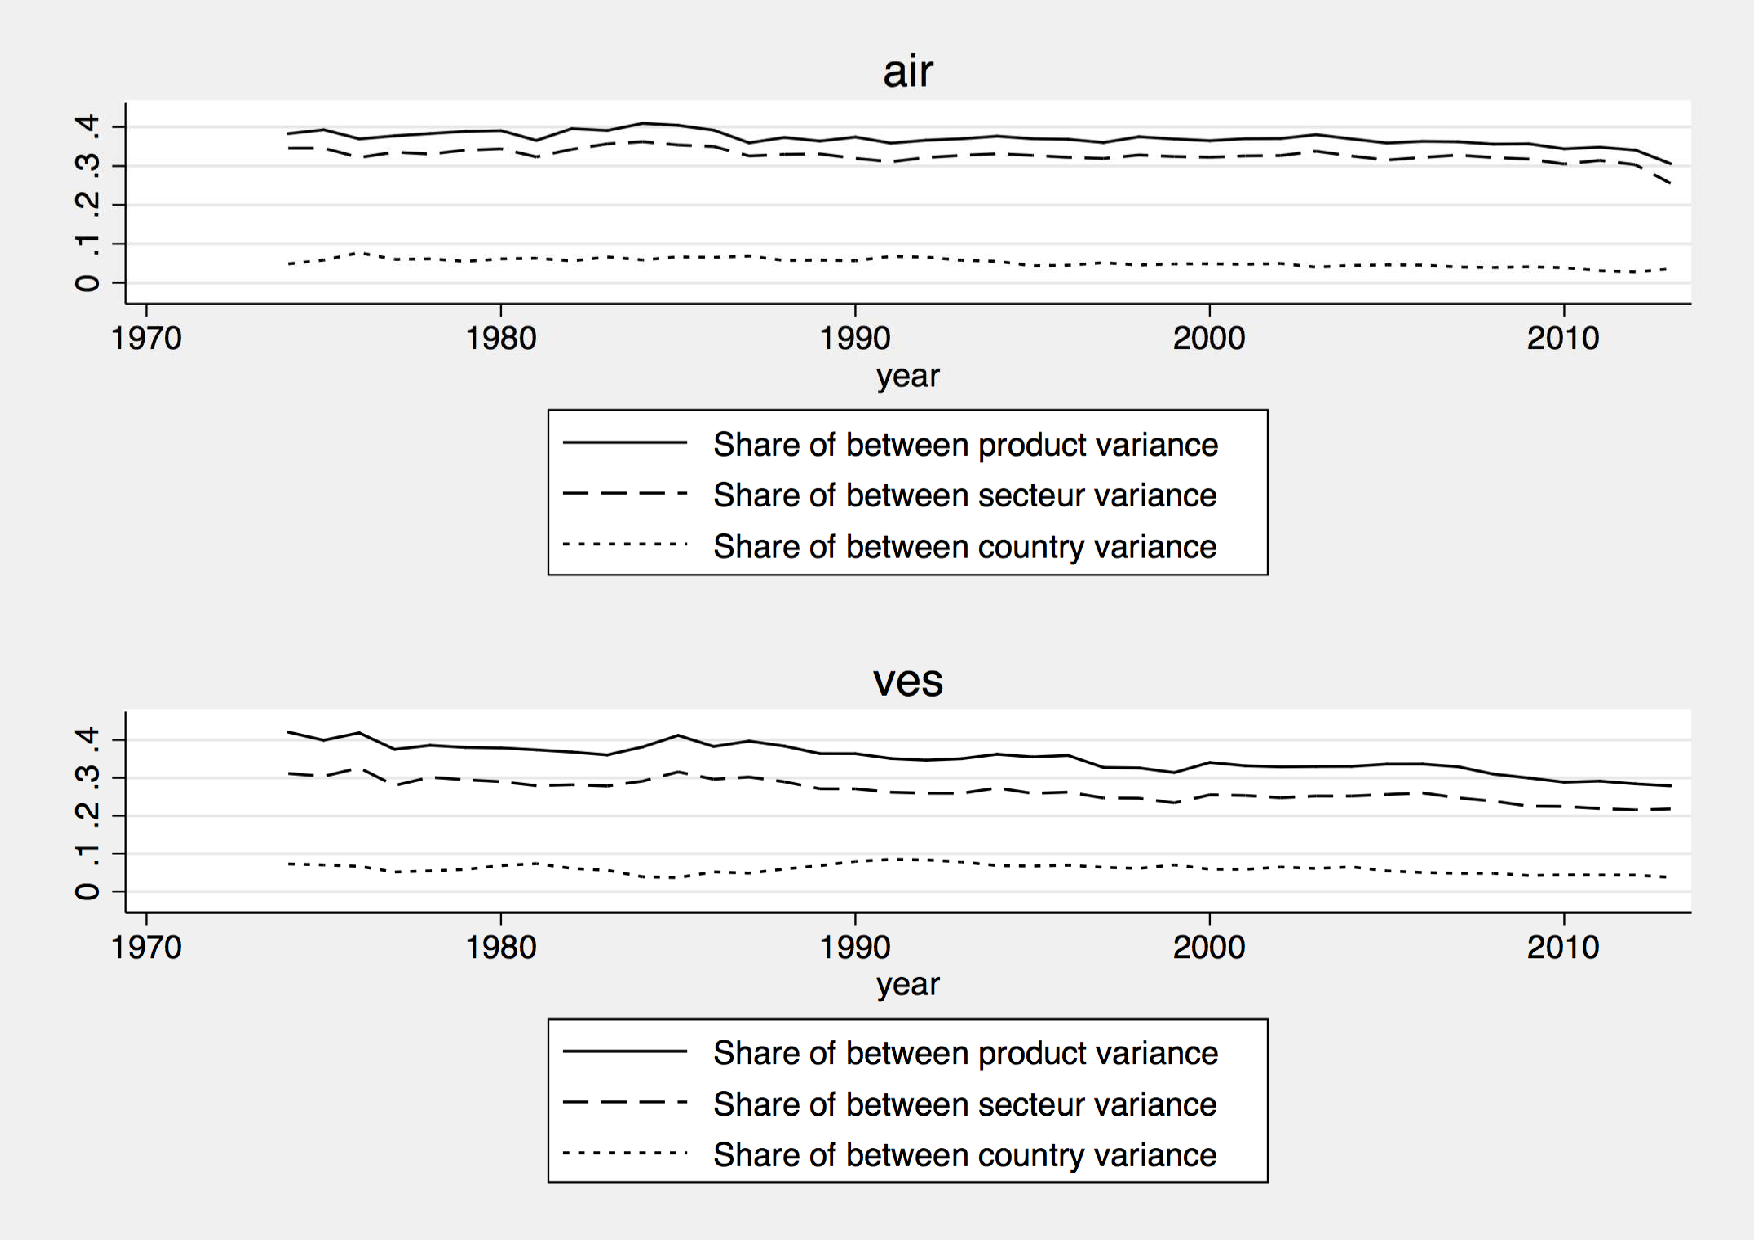
\includegraphics[width=10cm, height=7cm]{variance_decomposition.pdf}
%{\footnotesize {OECD data} }
\end{center}
\end{figure}

Two interesting results emerge from Figure \ref{fig:decomp_variance}. First, the share of the cif-fas price gap variance that comes from the variance between products (5-digit level) is of same magnitude of order at the variance between sectors at the 3-digit level. Both account for between 30 and 40\% of the total variance in Air transport, depending on the years considered. This is also the case for vessel transport, even if the difference between the between-product variance share and the between-sector share is more pronounced (30\% for the between-sector vs 40\% for the between-product variance at the beginning of the period). This delivers an indirect robustness check to the degree of classification we have retained to estimate international transport costs. Second, the variance of the cif-fas price gap that can be attributed to the product (or sector) dimension is much larger than the between-country variance. This holds throughout the period and for both transport modes. This suggests that what primarily matters in international transport costs is mostly attributable to the product \textit{per se}, rather than to the country where it comes from. By extension, one can expect a limited role of distance and other country-related variables as determinants of transport costs.

\section{Estimation at the 4-digit level \label{app:4digit}}

In this section, we report the estimation results when we retain the 4-digit classification level ($s$=4-digit).

\subsection{Transport cost estimates}


Tables \ref{tab:result_air_rob} and \ref{tab:result_ves_rob} report the estimates of both models (with and without additive costs) in Air and Ocean transport respectively.

\begin{table}[htbp]
  \centering
  \caption{Air: Transport costs estimates, Selected years, 4-digit}
\begin{center}
    \begin{tabular}{l|cccccc}
   \hline\hline
Year & 1974  & 1981  & 1989  & 2001  & 2009  & 2013 \\ \hline
\multicolumn{7}{l}{\textbf{Model (A) - With only Ad-Valorem TC} ($\widehat{\tau}^{ice}$, in \%) }  \\
\hline
Mean  & 6.6 & 5.8 & 5.2 & 3.3 & 3.7 & 3.2 \\
Median & 5.2 & 4.4 & 4.1 & 2.1 & 2.7 & 2.6 \\
%Standard Error & 0.056 & 0.054 & 0.046 & \multicolumn{1}{c}{0.040} & \multicolumn{1}{c}{0.036} & \multicolumn{1}{c}{0.025}  \\
\hline
\multicolumn{7}{l}{\textbf{Model (B) - With Additive \& Ad-Valorem TC}}  \\ \hline
\multicolumn{7}{l}{\textit{Ad-valorem term }($\widehat{\tau}^{adv}$, in \%) }   \\ \hline
Mean  & 3.5 & 2.6 & 3.1 & 1.5 & 2.1 & 1.6  \\
Median & 2.5 & 1.7 & 1.9 & 1.0 & 1.7 & 1.4  \\
%Standard Error & 0.036 & 0.028 & 0.030 & \multicolumn{1}{c}{0.021} & \multicolumn{1}{c}{0.024} & \multicolumn{1}{c}{0.015}  \\
\hline
\multicolumn{7}{l}{\textit{Additive term} ($\widehat{t}/\widetilde{p}$), in \%}    \\ \hline
Mean  & 2.6 & 2.1 & 1.7 & 1.2 &1.2 & 1.0 \\
Median & 1.2 & 0.6 & 0.6 & 0.5 & 0.4 & 0.4  \\
%Standard Error & 0.039 & 0.042 & 0.033 & \multicolumn{1}{c}{0.027} & \multicolumn{1}{c}{0.029} & \multicolumn{1}{c}{0.019} \\
\hline
\# observations & 14944 & 16844 & 25307 & \multicolumn{1}{c}{35005} & \multicolumn{1}{c}{38475} & \multicolumn{1}{c}{39460}  \\
\hline\hline
\multicolumn{7}{l}{\parbox[l]{11cm}{ \vspace{7pt}\scriptsize{Notes: TC = Transport Costs. Statistics are obtained weighting each observation by its value in transport (mode-dependent). Additive term expressed in fraction of fas price.}}}
\end{tabular}%
\end{center}
  \label{tab:result_air_rob}
\end{table}%


\begin{table}[htbp]
  \centering
\caption{Vessel: Transport costs estimates, Selected years, 4-digit}
\begin{center}
    \begin{tabular}{l|cccccc}
   \hline\hline
Year & 1974  & 1981  & 1989  & 2001  & 2009  & 2013 \\
\hline
\multicolumn{7}{l}{\textbf{Model (A) - With only Ad-Valorem TC} ($\widehat{\tau}^{ice}$, in \%)} \\
\hline
Mean  & 9.8 & 6.1 & 5.8 & 5.1 & 4.2 & 3.6  \\
Median & 9.4 & 5.1 & 4.8 & 4.5 & 3.8 & 3.1 \\
%Standard Error & 0.060 & 0.038 & \multicolumn{1}{c}{0.036} & \multicolumn{1}{c}{0.030} & \multicolumn{1}{c}{0.023} & \multicolumn{1}{c}{0.020} \\
\hline
\multicolumn{7}{l}{\textbf{Model (B) - With Additive \& Ad-Valorem TC} }\\ \hline
\multicolumn{7}{l}{\textit{Ad-valorem term} ($\widehat{\tau}^{adv}$, in \%) }   \\ \hline
Mean  & 5.4 & 3.4 & 2.8 & 2.8 & 2.4 & 2.1  \\
Median & 4.9 & 3.0 & 2.4 & 2.5 & 2.6 & 1.8 \\
%Standard Error & 0.043 & 0.026 & \multicolumn{1}{c}{0.025} & \multicolumn{1}{c}{0.021} & \multicolumn{1}{c}{0.016} & \multicolumn{1}{c}{0.013}  \\
\hline
\multicolumn{7}{l}{\textit{Additive term} ($\widehat{t}^{add}/\widetilde{p}$, in \%) }   \\ \hline
Mean  & 4.6 & 2.6 & 3.1 & 2.4 & 2.1 & 1.5  \\
Median & 2.9 & 1.3 & 1.9 & 1.5 & 1.3 & 0.8 \\
%Standard Error & 0.068 & 0.044 & \multicolumn{1}{c}{0.037} & \multicolumn{1}{c}{0.035} & \multicolumn{1}{c}{0.031} & \multicolumn{1}{c}{0.023} \\
\hline
\# observations & 19196 & 17916 & \multicolumn{1}{c}{29387} & \multicolumn{1}{c}{36677} & \multicolumn{1}{c}{37643} & \multicolumn{1}{c}{38820} \\
\hline\hline
\multicolumn{7}{l}{\parbox[l]{11cm}{ \vspace{7pt}\scriptsize{Notes: TC = Transport Costs. Statistics are obtained weighting each observation by its value in transport (mode-dependent). Additive term expressed in fraction of fas price.}}}
\end{tabular}%
\end{center}
\label{tab:result_ves_rob}%
\end{table}%

\subsection{Goodness-of-fit tests at the 4-digit level}

We now report the goodness-of-fit exercise (conducted by transport mode) at the 4-digit product classification level (for the selected years). The results are reported in Tables \ref{tab:good_fit_air_rob} (for Air) and \ref{tab:good_fit_ves_rob} (for Vessel).
\begin{table}[htbp]
  \centering
  \caption{Air: Measures of Goodness-of-fit, 4-digits}
\begin{center}
\label{tab:good_fit_air_rob}%
%\vspace{0.5cm}
%\scalebox{0.97}{
  \footnotesize{
\begin{tabular}{l|cccccc}
\hline
\hline
      & \multicolumn{6}{c}{Year}              \\
      & \multicolumn{1}{c}{1974} & \multicolumn{1}{c}{1981} & \multicolumn{1}{c}{1989} & \multicolumn{1}{c}{2001} & \multicolumn{1}{c}{2009} & \multicolumn{1}{c}{2013}  \\
\hline
\textbf{R2} & \multicolumn{1}{c}{} & \multicolumn{1}{c}{} & \multicolumn{1}{c}{} &       &       &      \\
Model (A)& \multicolumn{1}{c}{0.48} & \multicolumn{1}{c}{0.49} & \multicolumn{1}{c}{0.50} & \multicolumn{1}{c}{0.50} & \multicolumn{1}{c}{0.45} & \multicolumn{1}{c}{0.35} \\
Model (B) & \multicolumn{1}{c}{0.63} & \multicolumn{1}{c}{0.66} & \multicolumn{1}{c}{0.65} & \multicolumn{1}{c}{0.66} & \multicolumn{1}{c}{0.54} & \multicolumn{1}{c}{0.45} \\
\textbf{SER} & \multicolumn{1}{c}{} & \multicolumn{1}{c}{} & \multicolumn{1}{c}{} &       & \multicolumn{1}{c}{} & \multicolumn{1}{c}{}  \\
Model (A)& \multicolumn{1}{c}{0.8} & \multicolumn{1}{c}{0.9} & \multicolumn{1}{c}{0.83} &   0.87    & \multicolumn{1}{c}{0.88} & \multicolumn{1}{c}{0.93}  \\
Model (B) & \multicolumn{1}{c}{0.67} & \multicolumn{1}{c}{0.74} & \multicolumn{1}{c}{0.69} &  0.80     & \multicolumn{1}{c}{0.80} & \multicolumn{1}{c}{0.86}  \\
\textbf{Log-likelihood} & \multicolumn{1}{c}{} & \multicolumn{1}{c}{} & \multicolumn{1}{c}{} &       & \multicolumn{1}{c}{} & \multicolumn{1}{c}{} \\
Model (A) & \multicolumn{1}{c}{-17505.6} & \multicolumn{1}{c}{-21813.5} & \multicolumn{1}{c}{-30960.6} & \multicolumn{1}{c}{-44067.6} & \multicolumn{1}{c}{-49375.6} & \multicolumn{1}{c}{-53197.9}  \\
Model (B) & \multicolumn{1}{c}{-14895.8} & \multicolumn{1}{c}{-18589.9} & \multicolumn{1}{c}{-26553.5} & \multicolumn{1}{c}{-37297.9} & \multicolumn{1}{c}{-45747.6} & \multicolumn{1}{c}{-49899.1}  \\
\textbf{AIC criteria} & \multicolumn{1}{c}{} & \multicolumn{1}{c}{} & \multicolumn{1}{c}{} &       & \multicolumn{1}{c}{}  \\
Model (A)& \multicolumn{1}{c}{36243.1} & \multicolumn{1}{c}{44966.9} & \multicolumn{1}{c}{63417.1} & \multicolumn{1}{c}{89747.2} & \multicolumn{1}{c}{100317.13} & \multicolumn{1}{c}{107963.7} \\
Model (B) & \multicolumn{1}{c}{31873.6} & \multicolumn{1}{c}{39495.8} & \multicolumn{1}{c}{55777.1} & \multicolumn{1}{c}{77439.9} & \multicolumn{1}{c}{94059.1} & \multicolumn{1}{c}{102224.3}  \\
\textbf{Test LL} &       &       &       &       &       &       \\
2$\times$(ll(UR) -ll(R)) & \multicolumn{1}{c}{5219.5} & \multicolumn{1}{c}{6447.1} & \multicolumn{1}{c}{8814.1} & \multicolumn{1}{c}{13539.4} & \multicolumn{1}{c}{7256.0} & \multicolumn{1}{c}{6597.5}  \\
\# restrictions  & \multicolumn{1}{c}{640} & \multicolumn{1}{c}{698} & \multicolumn{1}{c}{778} & \multicolumn{1}{c}{833} & \multicolumn{1}{c}{824} & \multicolumn{1}{c}{818}  \\
p-value & \multicolumn{1}{c}{0.00} & \multicolumn{1}{c}{0.000} & \multicolumn{1}{c}{0.00} & \multicolumn{1}{c}{0.00} & \multicolumn{1}{c}{0.00} & \multicolumn{1}{c}{0.000} \\
\hline\hline
\multicolumn{7}{l}{\parbox[l]{13cm}{ \vspace{7pt}\scriptsize{Notes: Model (A) = with only ad-valorem transport costs. Model (B) = with additive \& ad-valorem
transport costs. R$^{2}$ between the log of predicted ratio and the log of the observed ratio. The number \# of restrictions is equal to the number of parameters estimated, i.e., the number of partner countries plus the number of products.}}}
\end{tabular}%
}
\end{center}
\end{table}%


\begin{table}[htbp]
  \centering
  \caption{Vessel: Measures of Goodness-of-fit, 4-digits}
\begin{center}
\label{tab:good_fit_ves_rob}%
  \footnotesize{
\begin{tabular}{l|cccccc}
\hline
\hline
      & \multicolumn{6}{c}{Year}                   \\
      & \multicolumn{1}{c}{1974} & \multicolumn{1}{c}{1981} & \multicolumn{1}{c}{1989} & \multicolumn{1}{c}{2001} & \multicolumn{1}{c}{2009} & \multicolumn{1}{c}{2013}  \\ \hline
\boldmath{}\textbf{R$^{2}$}\unboldmath{} &       &       &       &       &       &         \\
Term I only & 0.50  & 0.45  & \multicolumn{1}{c}{0.47} & \multicolumn{1}{c}{0.41} & \multicolumn{1}{c}{0.37} & \multicolumn{1}{c}{0.35} \\
Terms A \& I & 0.66  & 0.62  & \multicolumn{1}{c}{0.62} & \multicolumn{1}{c}{0.58} & \multicolumn{1}{c}{0.51} & \multicolumn{1}{c}{0.46} \\
\textbf{SER} &       &       & \multicolumn{1}{c}{} & \multicolumn{1}{c}{} & \multicolumn{1}{c}{} & \multicolumn{1}{c}{} \\
Model (A) &    0.58   &   0.64    & \multicolumn{1}{c}{0.61} & \multicolumn{1}{c}{0.0.72} & \multicolumn{1}{c}{0.79} & \multicolumn{1}{c}{0.82} \\
Model (B) &   0.48    &    0.53   & \multicolumn{1}{c}{0.51} & \multicolumn{1}{c}{0.61} & \multicolumn{1}{c}{0.69} & \multicolumn{1}{c}{0.75} \\
\textbf{Log-likelihood} &       &       & \multicolumn{1}{c}{} & \multicolumn{1}{c}{} & \multicolumn{1}{c}{} & \multicolumn{1}{c}{} \\
Model (A)& -16460.1 & -16951.6 & \multicolumn{1}{c}{-26771.4} & \multicolumn{1}{c}{-39008.3} & \multicolumn{1}{c}{-43888.9} & \multicolumn{1}{c}{-47161.6} \\
Model (B) & -12743.65 & -13546.9 & \multicolumn{1}{c}{-21752.8} & \multicolumn{1}{c}{-33281.0} & \multicolumn{1}{c}{-39078.9} & \multicolumn{1}{c}{-43399.2}  \\
\textbf{AIC criteria} &       &       & \multicolumn{1}{c}{} & \multicolumn{1}{c}{} & \multicolumn{1}{c}{} & \multicolumn{1}{c}{} \\
Model (A) & 34464.2 & 35491.2 & \multicolumn{1}{c}{55272.9} & \multicolumn{1}{c}{79800.7} & \multicolumn{1}{c}{89459.8} & \multicolumn{1}{c}{95987.2}\\
Model (B) & 28271.3 & 29877.8 & \multicolumn{1}{c}{46595.6} & \multicolumn{1}{c}{69743.9} & \multicolumn{1}{c}{81155.7} & \multicolumn{1}{c}{89692.4} \\
\textbf{Test LL} &       &       & & &  & \\
2$\times$(ll(UR) -ll(R)) & 12385.80 & 11226.8 & \multicolumn{1}{c}{17354.7} & \multicolumn{1}{c}{20113.5} & \multicolumn{1}{c}{16608.2} & \multicolumn{1}{c}{12589.6} \\
\# restrictions  & 797   & 814   & \multicolumn{1}{c}{881} & \multicolumn{1}{c}{910} & \multicolumn{1}{c}{886} & \multicolumn{1}{c}{874} \\
p-value & 0.000 & 0.000 & \multicolumn{1}{c}{0.000} & \multicolumn{1}{c}{0.000} & \multicolumn{1}{c}{0.000} & \multicolumn{1}{c}{0.000} \\
\hline\hline
\multicolumn{7}{l}{\parbox[l]{13cm}{ \vspace{7pt}\scriptsize{Notes: Model (A) = with only ad-valorem transport costs. Model (B) = with additive \& ad-valorem
transport costs. R$^{2}$ between the log of predicted ratio and the log of the observed ratio. The number \# of restrictions is equal to the number of parameters estimated, i.e., the number of partner countries plus the number of products.}}}
\end{tabular}%
}
\end{center}
\end{table}%


\section{Eliminating the composition effects: More details \label{app:comp-effects}}

In this section, we explain in more details the method employed to eliminate the country- and product- dimensions of the estimated transport cost.

\subsection{More on our methodology}


\subsubsection{Additive and ad-valorem transport costs: Excluding the composition effects}

In this section, we detail our methodology to extract the time trend in the ``ceteris paribus'' (or fitted) transport cost component, for each the ad-valorem and the additive component.

\paragraph{For the ad-valorem component} Consider first the multiplicative transport cost component. Rewriting Equation (\ref{eq:compeffects_mult}) by taking the exponential, we get:

\begin{equation*}
\widehat{\tau}_{ikt}=\exp\left(\delta + \sum_{i \neq \text{AFG}}\alpha_i.\mathbb{1}_i+\sum_{k\neq \text{011}}\beta_k.\mathbb{1}_k\right).\exp\left(\sum_{t \neq 1974}\gamma_t.\mathbb{1}_t\right) .\exp\left(\epsilon_{ikt}\right)
\end{equation*}

Based on this equation, we deduce after estimation that:
\begin{eqnarray*}
\text{For the year 1974}&& \widehat{\tau}_{is74} = \exp(\delta +\alpha_i+\beta_s), \\
\text{For any year}~t> 1974&& \widehat{\tau}_{ist} = \exp(\delta +\alpha_i+\beta_s)\times \exp(\gamma_t)
\end{eqnarray*}

From this, we obtain the following recursive link: $\widehat{\tau}_{ist} = \widehat{\tau}_{is74}\exp(\gamma_t)$. Given that $\tau >1$, we can rewrite to get the percentage change between year 1974 and any year $t>1974$:
\begin{equation*}
\Gamma_{ist} = 100.\frac{\widehat{\tau}_{ist}-1}{\widehat{\tau}_{is74}-1} = 100.\frac{\widehat{\tau}_{is74}\exp(\gamma_t)-1}{\widehat{\tau}_{is74}-1}
\end{equation*}

As such, the index of transport costs in year $t$ (relative to the reference year 1974) $\Gamma_{ist} $  only depends on the cost observed in 1974 and the time trend. At this stage though, it remains specific to a product-origin country pair. Next step is to build the index $\Gamma^{adv}_t$ such that:
\begin{equation}
 \Gamma^{adv}_t= 100\frac {\bar{\tau}_{1974}.\exp(\gamma_t)-1} {\bar{\tau}_{1974}-1}  \label{eq:tcadv_compoeffect}
\end{equation}
\noindent that is, Equation (\ref{eq:comp_effects_adv}) with $\bar{\tau}_{1974} = \exp(\delta + \sum_i \alpha_i + \sum_k \beta_k$) the mean (ad-valorem) transport cost in 1974.

\paragraph{For the additive component} After estimating Equation (\ref{eq:compeffects_add}), we can re-build the additive component according to:
\begin{eqnarray*}
\text{For the year 1974}&&\widehat{t}_{is74}=  \delta + \alpha_i+ \beta_s, \\
\text{For any year}~t> 1974&&\widehat{t}_{ist}=\left(\delta + \alpha_i+ \beta_s\right).\exp(\gamma_t)
\end{eqnarray*}

From this, we deduce the recursive link: $\widehat{t}_{ist} = \widehat{t}_{is74} \times \exp(\gamma_t)$. Given the constraint $t>0$, we then obtain the percentage change from 1974 from:

\begin{equation}
\Gamma^{add}_{ist} = 100\frac{\widehat{t}_{ist}}{\widehat{t}_{ik74}} = 100\exp(\gamma_t) \label{eq:indice_add}
\end{equation}

\noindent Note that it is independent of the product-origin country pair, we can thus rewrite the time-trend series for the additive transport cost component as:
\begin{equation}
\Gamma^{add}_t  = 100\exp(\gamma_t) \label{eq:tcadd_compoeffect}
\end{equation}

\paragraph{Obtaining the unfitted measures} It consists in expressing the unfitted transport cost component as as index, with reference value 100 in 1974, starting from the estimated values previously obtained ($\widehat{\tau}_t$, $\widehat{t}_t$, for each year $t$ from 1974 to 2013). That is, we apply the simple formula to get the following indices, for the ad-valorem and the additive cost components respectively:

$$\Gamma^{adv, raw}_t = 100\times\frac{\widehat{\tau}_t}{\widehat{\tau}_{1974}},\qquad \Gamma^{add, raw}_t = 100\times\frac{\widehat{t}_t}{\widehat{t}_{1974}}$$

\subsubsection{For the total cost measure}

We also build a measure of the ``overall'' transport costs, that agglomerates our estimates of the two additive and iceberg components. We construct this measure (by transport mode) on both the unfitted series and the ``pure'' transport cost series (composition effects excluded). Even if obeying to the same logic, we proceed slightly differently for the unfitted and the fitted measures though, as we now explain.\smallskip

For the unfitted measure, based on Equation (\ref{eq:base_estimee}), we build for each transport mode, the ``overall'' transport cost as:
$$\widehat{tc}^{raw}_t= \widehat{\tau}^{adv}_t -1 + \widehat{t}_t$$
\noindent where $\widehat{\tau}^{adv}_t$ and $\widehat{t}_t$ have been estimated (by year) as explained in Section \ref{sec:data_method}, $\widehat{\tau}^{adv}_t-1$ measuring the ad-valorem transport cost component and $\widehat{t}_t$ the additive component, both expressed in percentage of the fas price. For sake of comparison, we transform this ``overall'' transport cost in an index with basis year 1974, applying a similar formula as above (by transport mode):
$$\Gamma^{tc, raw}_t = 100\frac{\widehat{tc}^{raw}_t -1 }{\widehat{tc}^{raw}_{1974}-1}$$

We apply the same logic to construct the fitted measure of total transport cost (i.e., composition effect excluded), with a first step that consists in getting the fitted measures of each transport cost component in value (rather than as an index). For the ad-valorem component, this can be obtained starting from Equation (\ref{eq:tcadv_compoeffect}), rewritten to get:

$$\widehat{\tau}^{cp, adv}_t = \frac{\Gamma^{adv}_t \left(\bar{\tau}_{1974}-1\right)}{100} +1$$

with $\widehat{\tau}^{cp, adv}_t \equiv \bar{\tau}_{1974}.\exp(\gamma_t)$ the yearly value of the \textit{ceteris paribus} (fitted) ad-valorem cost. A similar reasoning starting from Equation (\ref{eq:tcadd_compoeffect}) gives the fitted value for the additive cost component as:

$$\widehat{t}^{cp}_t = \frac{\Gamma^{add}_t}{100}$$

with $\widehat{t}^{cp}_t \equiv \exp(\gamma_t)$ the yearly value of the \textit{ceteris paribus} (fitted) additive cost.


We then deduce the fitted value of the overall cost according to:
$$\widehat{tc}^{cp}_t= \widehat{\tau}^{cp, adv}_t  + \widehat{t}^{cp}_t$$

Last, we transform this (fitted) ``overall'' transport cost in an index with basis year 1974, applying a similar formula as above (by transport mode):
$$\Gamma^{tc}_t = 100\frac{\widehat{tc}^{cp}_t -1 }{\widehat{tc}^{cp}_{1974}-1}$$

This finally leaves us with six time series, all built as indices with the reference value 100 in 1974: Three time series for the unfitted transport costs measures $\{\Gamma^{add, raw}_t, \Gamma^{adv, raw}_t, \Gamma^{tc, raw}_t \}$  (additive, ad-valorem and overall resp.), and three series for the fitted values $\{\Gamma^{add}_t, \Gamma^{adv}_t, \Gamma^{tc}_t \}$ (additive, ad-valorem and overall respectively).

\subsection{Comparing with \cite{hummels2007} \label{app:compare_Hummels}}

In this section, we investigate the difference of results with \cite{hummels2007} regarding the importance of the composition effects in characterizing the time trends of international transport costs. In order to do so, we start from the empirical specification implemented by \cite{hummels2007} (also making use of Hummels' Stata codes provided on his webpage\footnote{\url{http://www.krannert.purdue.edu/faculty/hummelsd/research/jep-transport-cost-data.php}}), to better identify the precise points of difference between our estimation strategies.

Let us start from Hummels' (2007) quotation (p. 146) according to which (for air), the ``\textit{unadjusted measure of ad valorem air shipping costs [is] the aggregate expenditures on air shipping divided by the value of airborne imports}''. From this, we get the ``raw'' ad-valorem measure of transport costs as the ratio between the imported total value and the exported total value ($(p_{ikt} - \widetilde{p}_{ikt})q_{ikt}/\widetilde{p}_{ikt}q_{ikt})$, the mean yearly value being obtained by weighting each flow by its value in total trade flows (ie, yielding the observed aggregate value of $\tau_t$ for air).

Consider now the ``fitted ad-valorem rate''. \cite{hummels2007} uses ``\textit{a regression in which the dependent variable is the ad-valorem air freight cost in logs for commodity $k$ shipped from exporter} $i$\footnote{To be consistent with our notations, we change the country subscript from $j$ (Hummels' (2007) terminology) to $i$ (our terminology).} \textit{at time $t$. The independent variables include a separate intercept for each exporter-commodity shipped, the weight/value ratio in logs for each shipment, and year dummy variables}''. With the value of the shipment equal to $\widetilde{p}_{ikt}q_{ikt}$, and denoting the air freight cost as $TC_{ikt}$, we can formulate the above sentence according to the following equation (suppressing the transport mode index to alleviate notation):

\begin{eqnarray}
&&\ln TC_{ikt} = \delta+ \beta \ln \frac{q_{ikt}}{\widetilde{p}_{ikt}q_{ikt}} + \sum_{i,k}\alpha_{ik}.\mathbb{1}_{ik}+ \sum_{t}\gamma_{t}.\mathbb{1}_{t} + \epsilon_{ikt} \notag \\
\Leftrightarrow && \ln TC_{ikt} = \delta+ \beta \ln \frac{1}{\widetilde{p}_{ikt}} + \sum_{i,k}\alpha_{ik}.\mathbb{1}_{ik}+ \sum_{t}\gamma_{t}.\mathbb{1}_{t} + \epsilon_{ikt} \label{eq:Hummels1}
\end{eqnarray}

\noindent where $TC_{ikt}$ is measured by the ratio between (air) charges, i.e. $(p_{ikt} - \widetilde{p}_{ikt})q^{fas}_{ikt}$ and the value of the shipment, i.e. $\widetilde{p}_{ikt}q^{fas}_{ikt}$, or equivalently : $TC_{ikt} = \frac{p_{ikt} - \widetilde{p}_{ikt}}{\widetilde{p}_{ikt}}$.\medskip

After estimating Equation (\ref{eq:Hummels1}), \cite{hummels2007} uses the predicted value of the regression, denoted $\widehat{TC}_{ikt}$, to obtain the unweighed average in the product/origin country dimension $i,k$, that is $\widehat{TC}_{t}$, to be compared to the unfitted ad-valorem rate $TC_{t}$ (by transport mode).\medskip

What are the main differences with our estimation strategy? Five points may be underlined. First, \cite{hummels2007} obtains the fitted ad-valorem rate in one step (considering the observed export-import price gap on the left-hand side of Equation (\ref{eq:Hummels1})), while we use our two-step approach to extract the fitted transport cost (ie, composition effect excluded) from the (already estimated) unfitted rate. However, this is a slight difference, as in both cases it ultimately amounts taking the predicted value of Equation (\ref{eq:Hummels1}) (which eliminates the changes specific to the origin country/product/year triplet).

A second minor difference is that we separate the country-product fixed effects ($\sum_{i,k}\alpha_{ik}.\mathbb{1}_{ik}$ in Equation (\ref{eq:Hummels1})) in two separate components (origin country and product dimensions). As discussed in Section \ref{sec:robustness}, this is constrained by the number of fixed effects to estimate. However, we do not view this as the major cause of difference between our tow methods, as it can be inferred from the robustness analysis on this point in Section \ref{sec:robustness}.

Third, in contrast to us, \cite{hummels2007} does not purge its measure of the fitted ad-valorem rate by the country-sector fixed effects. This is not likely to make a substantial difference though, as these fixed effects are by nature constant over time. Accordingly, they only play as a scale effect as the estimate is in log. Fourth, we differ in the weighting scheme retained to obtain the yearly value of the fitted transport cost (in the terms of \citeh{hummels2007} method, the switch from $\widehat{TC}_{ikt}$ to $\widehat{TC}_{t}$, Equations (\ref{eq:comp_effects_adv}) and (\ref{eq:comp_effects_add}) in our case). \cite{hummels2007} takes the unweighed average value over the $i,k$ dimension, which implicitly attributes a weight equal to 1 to each flow. We proceed differently, as we weight each flow by its relative value on total trade flows observed in 1974. This choice is made for two reasons. First, this weighting scheme does not overweight the small flows in value. Second, considering the 1974 weighting scheme makes sense as starting point of our time trend analysis. However, we ensure that our results are not sensitive to an alternative weighting scheme, by building the average fitted transport costs rate as in \cite{hummels2007}, as reported in Section \ref{sec:robustness}.

One last difference remains to be commented, which relies on the way the additive component of international transport costs is treated. As we show below, it turns out to be key in accounting for the difference of results with \cite{hummels2007}. Coming back to Equation (\ref{eq:Hummels1}), it can be shown that it encompasses the two extreme cases of only ad-valorem costs ($\beta = 0$) and only additive costs ($\beta=1$), as also pointed out in \cite{hummels_skiba}. To see it clearly, rewrite Equation (\ref{eq:Hummels1}) in a simpler form as:

$$\ln TC_{ikt} \equiv \ln \left(\frac{p_{ikt}- \widetilde{p}_{ikt}}{\widetilde{p}_{ikt}} \right) = \Delta_{ikt}- \beta \ln \widetilde{p}_{ikt} $$

\noindent with $\Delta_{ikt} \equiv \sum_{i,k}\alpha_{ik}.\mathbb{1}_{ik}+ \sum_{t}\gamma_{t}.\mathbb{1}_{t}$ agglomerates the various fixed effects for reading clarity.

Under the first polar case with $\beta = 1$, it becomes:
\begin{eqnarray*}
&&\ln \left(\frac{p_{ikt}- \widetilde{p}_{ikt}}{\widetilde{p}_{ikt}} \right) = \Delta_{ikt}- \ln \widetilde{p}_{ikt} \\
\Leftrightarrow && \ln (p_{ikt}- \widetilde{p}_{ikt}) = \Delta_{ikt} \\
\end{eqnarray*}
\noindent Equivalently, we can write:

\begin{eqnarray*}
&&p_{ikt} = \widetilde{p}_{ikt} + \exp(\Delta_{ikt})\\
\Leftrightarrow && p_{ikt} = \widetilde{p}_{ikt} + t_{ikt}
\end{eqnarray*}
\noindent with $t_{ikt}$ appropriately defined. This exactly corresponds to the case of additive costs only.

In the second polar case with $\beta = 0$, Equation (\ref{eq:Hummels1}) becomes:
\begin{eqnarray*}
&&\ln \left(\frac{p_{ikt}- \widetilde{p}_{ikt}}{\widetilde{p}_{ikt}} \right) = \Delta_{ikt} \\
\Leftrightarrow && \ln \left(\frac{p_{ikt}}{\widetilde{p}_{ikt}}-1\right) = \Delta_{ikt}\\
\Leftrightarrow && \frac{p_{ikt}}{\widetilde{p}_{ikt}}  = \exp (\Delta_{ikt})+1
\end{eqnarray*}
\noindent that is,

$$p_{ikt} = \tau_{ikt} \widetilde{p}_{ikt}$$

\noindent with $\tau_{ikt}$ appropriately defined. This exactly corresponds to the case of ad-valorem transport costs only.


As noted by \cite{hummels_skiba}, $0<\beta<1$ represents the elasticity of freight costs to the export prices, increasing with the relative weight of the additive component in international transport costs. By estimating Equation (\ref{eq:Hummels1}) with a constant $\beta$, \cite{hummels2007} assumes that the share of additive costs does not vary over time, country partner or product. This is an important difference with our method, as we measure transport costs by explicitly allowing for an additive component that varies in the three dimensions (ie, somehow allowing for a varying $\beta$ across time, country partner and product). To establish this point clearly, we replicate the method adopted by \cite{hummels2007} exposed above on our database (which is the same as his until 2004). The results are reported in Figure \ref{fig:comp_effects_as_in_Hummels}.






\end{document}

